\documentclass[
]{jss}

\usepackage[utf8]{inputenc}

\providecommand{\tightlist}{%
  \setlength{\itemsep}{0pt}\setlength{\parskip}{0pt}}

\author{
Mladen Jovanović\\University of Belgrade \And Jason D. Vescovi\\University of Toronto
}
\title{\pkg{shorts}: An R Package for Modeling Short Sprints}

\Plainauthor{Mladen Jovanović, Jason D. Vescovi}

\Abstract{
Short sprint performance is one of the most distinguishable and admired physical trait in sports. Short sprints have been modeled using the mono-exponential equation that involves two parameters: (1) maximum sprinting speed (MSS) and (2) relative acceleration (TAU). The most common methods to assess short sprint performance are with a radar gun or timing gates. In this paper, we: 1) provide the \pkg{shorts} package that can model sprint timing data from these two sources; 2) discuss potential issues with assessing sprint time (synchronization and flying start, respectively); and 3) provide model definitions within the \pkg{shorts} package to help alleviate errors within the subsequent parameter outcomes.
}

\Keywords{sprinting, sports, modeling}

%% publication information
%% \Volume{50}
%% \Issue{9}
%% \Month{June}
%% \Year{2012}
%% \Submitdate{}
%% \Acceptdate{2012-06-04}

\Address{
    Mladen Jovanović\\
    University of Belgrade\\
    Faculty of Sport and Physical Education\\
Belgrade, Serbia\\
  E-mail: \email{coach.mladen.jovanovic@gmail.com}\\
  
      Jason D. Vescovi\\
    University of Toronto\\
    Faculty of Kinesiology and Physical Education\\
Graduate School of Exercise Science\\
Toronto, ON Canada\\
  E-mail: \email{vescovij@gmail.com}\\
  
  }


% Pandoc header

\usepackage{amsmath}

\begin{document}

\hypertarget{introduction}{%
\section{Introduction}\label{introduction}}

Short sprint performance is one of the most distinguishable and admired physical trait in sports. Short sprints, commonly performed in most team sports (e.g., soccer, field hockey, handball, football, etc.), are defined as maximal running from a stand still position over a distance that doesn't result in deceleration at the end. Peak anaerobic power is achieved within the first few seconds (\textless5s) of maximal efforts \citep{mangineSpeedForcePower2014}, whereas the ability to achieve maximal sprint speed varies based on the type of sport. For example, track and field sprinters are trained to achieve maximal speed later in a race (i.e., 50-60m) \citep{ward-smithEnergyConversionStrategies2001}, but team sport athletes have sport-specific attributes and reach it much sooner (i.e., 30-40m)\citep{brownAssessmentLinearSprinting2004}. Regardless of the differences in kinematics between athletes, evaluating short sprint performance is routinely included within a battery of fitness tests for a wide range of sports

The use of force plates is considered the gold standard for assessing mechanical properties of sprinting; however, there are logistical and financial challenges to capturing the profile of an entire sprint \citep{morinSimpleMethodComputing2019, samozinoSimpleMethodMeasuring2016}. Radar and laser technology are frequently used laboratory-grade methods \citep{buchheitMechanicalDeterminantsAcceleration2014, edwardsSprintAccelerationCharacteristics2020, jimenez-reyesRelationshipVerticalHorizontal2018, marcote-pequenoAssociationForceVelocity2019} but not normally accessible to practitioners working in sports. Undoubtedly, the most common method available and used to evaluate sprint performance are timing gates. Often multiple gates are positioned at varying distances to capture split times (e.g., 5, 10, 20m), which can now be incorporated into the method for determining sprint mechanical properties \citep{morinSimpleMethodComputing2019, samozinoSimpleMethodMeasuring2016}. This approach presents an advantage to practitioners who can use the outcomes to describe individual differences, quantify the effects of training interventions, and better understanding the limiting factors of performance. The \pkg{shorts} package \citep{R-shorts}, written in the R language \citep{R-base}, represents an open-source tool to help sport scientists translate raw timing data into detailed mechanical outcomes through mathematical modeling \citep{morinSimpleMethodComputing2019, samozinoSimpleMethodMeasuring2016}.

In the current paper, we will provide an explanation of one commonly used mathematical equation to model short sprints, modeling applications using the \pkg{shorts} package, issues that can arise during measurement and estimation, and potential solutions to those problems.

\hypertarget{mathematical-model}{%
\section{Mathematical model}\label{mathematical-model}}

Short sprints have been modeled using the mono-exponential equation \eqref{eq:velocity-time} originally proposed by \citet{doi:10.1098/rspb.1927.0035}, and more recently popularized by \citet{clarkNFLCombine40Yard2017}, and \citet{samozinoSimpleMethodMeasuring2016}. Equation \eqref{eq:velocity-time} represents function for instantaneous horizontal velocity \(v\) given the time \(t\) and two model parameters:

\begin{equation}
  v(t) = MSS \times (1 - e^{-\frac{t}{TAU}}) \label{eq:velocity-time}
\end{equation}

The parameters of the equation \eqref{eq:velocity-time} are \textit{maximum sprinting speed} (MSS; expressed in \(ms^{-1}\)) and \textit{relative acceleration} (TAU). Mathematically, TAU represents the ratio of MSS to initial acceleration (MAC; \textit{maximal acceleration}, expressed in \(ms^{-2}\)) \eqref{eq:maximal-acceleration}.

\begin{equation}
  MAC = \frac{MSS}{TAU}\label{eq:maximal-acceleration}
\end{equation}

Although TAU is used in the equations, and later estimated, it is preferred to use MAC instead since it is easier to grasp, particularly for less math inclined coaches.

By derivating equation \eqref{eq:velocity-time}, we can get equation for horizontal acceleration \eqref{eq:acceleration-time}.

\begin{equation}
  a(t) = \frac{MSS}{TAU} \times e^{-\frac{t}{TAU}}  \label{eq:acceleration-time}
\end{equation}

By integrating equation \eqref{eq:velocity-time}, we can get equation for distance covered \eqref{eq:distance-time}.

\begin{equation}
  d(t) = MSS \times (t + TAU \times e^{-\frac{t}{TAU}}) - MSS \times TAU  \label{eq:distance-time}
\end{equation}

Let's consider four athletes with different levels of MSS (high versus low maximal sprinting speed) and MAC (high versus low maximal acceleration; as mentioned previously, using MAC is preferred over using TAU) (Table \ref{tab:four-athletes-table}).

\begin{CodeChunk}
\begin{table}

\caption{\label{tab:four-athletes-table}Four athletes with different MSS and MAC parameters.}
\centering
\begin{tabular}[t]{l|r|r|r}
\hline
Athlete & MSS & MAC & TAU\\
\hline
Athlete A & 12 & 10 & 1.20\\
\hline
Athlete B & 12 & 6 & 2.00\\
\hline
Athlete C & 8 & 10 & 0.80\\
\hline
Athlete D & 8 & 6 & 1.33\\
\hline
\end{tabular}
\end{table}

\end{CodeChunk}

Figure \ref{fig:four-athletes-kinematics} depicts distance, velocity, and acceleration over time (from 0 to 6s).

\begin{CodeChunk}
\begin{figure}

{\centering 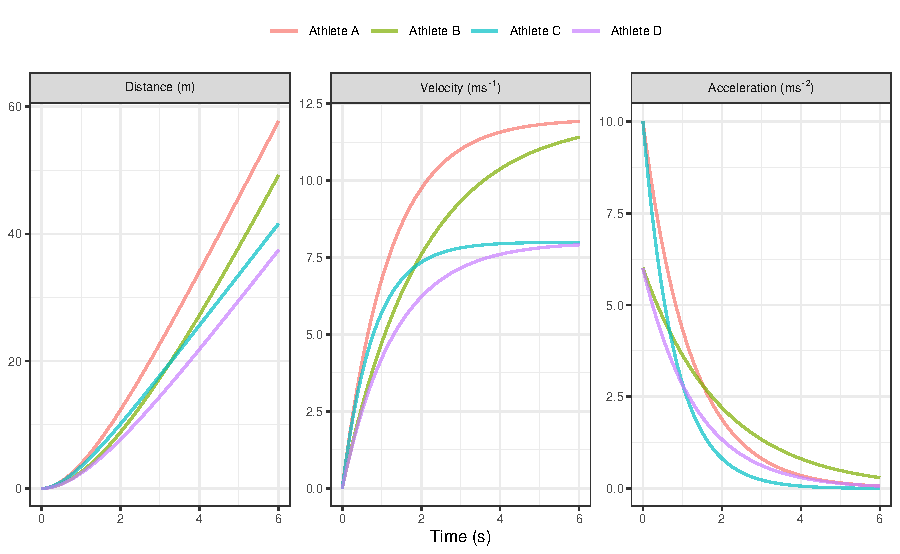
\includegraphics[width=1\linewidth]{paper_files/figure-latex/four-athletes-kinematics-1} 

}

\caption[Kinematic characteristic of four athletes with different MSS and MAC parameters over a period of 0 to 6seconds]{Kinematic characteristic of four athletes with different MSS and MAC parameters over a period of 0 to 6seconds.}\label{fig:four-athletes-kinematics}
\end{figure}
\end{CodeChunk}

Plotting acceleration against velocity (Figure \ref{fig:four-athletes-profile}), we will get Acceleration-Velocity profile, which is linear, according to the mathematical model.

\begin{CodeChunk}
\begin{figure}

{\centering 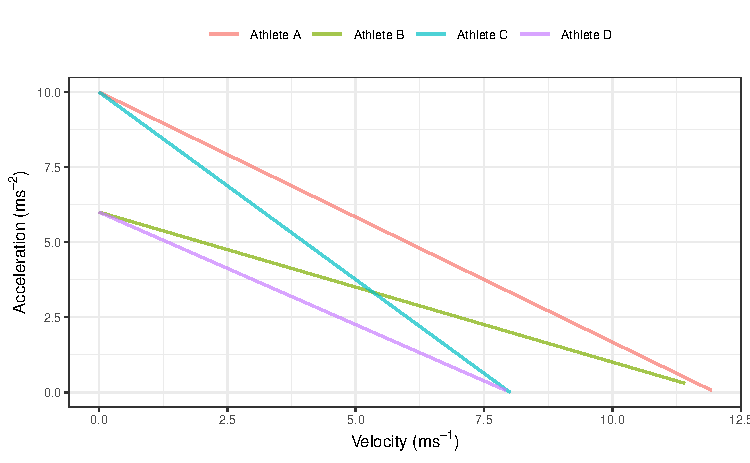
\includegraphics[width=1\linewidth]{paper_files/figure-latex/four-athletes-profile-1} 

}

\caption[Acceleration-Velocity profile of four athletes with different MSS and MAC parameters]{Acceleration-Velocity profile of four athletes with different MSS and MAC parameters.}\label{fig:four-athletes-profile}
\end{figure}
\end{CodeChunk}

\hypertarget{estimation-using-shorts-package}{%
\section{Estimation using shorts package}\label{estimation-using-shorts-package}}

Short sprints profiling is usually performed by: (1) measuring split times using timing gates (i.e., positioned at various distances, e.g., 5, 10, 20, 30, 40m), (2) getting a velocity trace using a radar gun. Estimation of MSS and TAU parameters from equation \eqref{eq:velocity-time} is performed in \pkg{shorts} package using non-linear least squares regression implemented in the \texttt{nls} function in the \pkg{base} R \citep{R-base} and \texttt{nlme} function in the \pkg{nlme} package \citep{R-nlme} for the mixed-effect models.

\hypertarget{estimating-short-sprint-parameters-using-split-times}{%
\subsection{Estimating short sprint parameters using split times}\label{estimating-short-sprint-parameters-using-split-times}}

Let's consider an example of an athlete with MSS equal to 9 \(ms^-1\), TAU equal to 1.3, and MAC equal to 6.92 \(ms^-2\) performing 40m sprint with timing gates positioned at each 10m split. For split times, distance is a predictor, and time is the outcome variable, thus the equation \eqref{eq:velocity-time} becomes:

\begin{equation}
  t(d) = TAU \times W(-e^{\frac{-d}{MSS \times TAU}} - 1) + \frac{d}{MSS} + TAU \label{eq:time-distance}
\end{equation}

\(W\) in equation \eqref{eq:velocity-time} represents Lambert's W function \citep{R-LambertW}. MSS and TAU parameters are estimated using \texttt{model\_using\_splits} function:

\begin{CodeChunk}
\begin{CodeInput}
R> require(shorts)
R> 
R> split_distance <- c(10, 20, 30, 40)
R> 
R> split_time <- c(2.17, 3.43, 4.60, 5.73)
R> 
R> m1 <- model_using_splits(
+   distance = split_distance,
+   time = split_time
+ )
R> 
R> m1
\end{CodeInput}
\begin{CodeOutput}
#> Estimated model parameters
#> --------------------------
#>                 MSS                 TAU                 MAC 
#>                9.01                1.31                6.89 
#>                PMAX     time_correction distance_correction 
#>               15.52                0.00                0.00 
#> 
#> Model fit estimators
#> --------------------
#>       RSE R_squared    minErr    maxErr maxAbsErr      RMSE       MAE 
#>   0.00249   1.00000  -0.00178   0.00265   0.00265   0.00176   0.00157 
#>      MAPE 
#>   0.04742
\end{CodeOutput}
\end{CodeChunk}

Maximal relative power (PMAX) from the output is estimated using \(\frac{MSS \times MAC}{4}\), which disregards the air resistance. \texttt{time\_correction} and \texttt{distance\_corection} parameters will be covered later in the article.

Besides providing \emph{residual standard error} (RSE), \pkg{shorts} functions provide additional model fit estimators. Additional information can be gained by exploring the returned object, particularly object returned from the \texttt{nls} function:

\begin{CodeChunk}
\begin{CodeInput}
R> summary(m1$model)
\end{CodeInput}
\begin{CodeOutput}
#> 
#> Formula: corrected_time ~ TAU * I(LambertW::W(-exp(1)^(-distance/(MSS * 
#>     TAU) - 1))) + distance/MSS + TAU
#> 
#> Parameters:
#>     Estimate Std. Error t value Pr(>|t|)    
#> MSS   9.0121     0.0155     581  3.0e-06 ***
#> TAU   1.3083     0.0066     198  2.5e-05 ***
#> ---
#> Signif. codes:  0 '***' 0.001 '**' 0.01 '*' 0.05 '.' 0.1 ' ' 1
#> 
#> Residual standard error: 0.00249 on 2 degrees of freedom
#> 
#> Number of iterations to convergence: 4 
#> Achieved convergence tolerance: 3.11e-06
\end{CodeOutput}
\end{CodeChunk}

Once we have estimated MSS and TAU, we can use \texttt{predict\_} family of functions to predict various relationships (i.e.~time at distance, acceleration at distance, velocity at time):

\begin{CodeChunk}
\begin{CodeInput}
R> # Predict time at distance
R> predict_time_at_distance(
+   distance = split_distance,
+   MSS = m1$parameters$MSS,
+   TAU = m1$parameters$TAU
+ )
\end{CodeInput}
\begin{CodeOutput}
#> [1] 2.17 3.43 4.60 5.73
\end{CodeOutput}
\begin{CodeInput}
R> 
R> # Predict acceleration at time
R> predict_acceleration_at_time(
+   time = c(0, 1, 2, 3, 4, 5, 6),
+   MSS = m1$parameters$MSS,
+   TAU = m1$parameters$TAU
+ )
\end{CodeInput}
\begin{CodeOutput}
#> [1] 6.8884 3.2075 1.4935 0.6954 0.3238 0.1508 0.0702
\end{CodeOutput}
\end{CodeChunk}

\hypertarget{air-resistance-and-the-calculation-of-force-and-mechanical-power}{%
\subsubsection{Air resistance and the calculation of force and mechanical power}\label{air-resistance-and-the-calculation-of-force-and-mechanical-power}}

To estimate force production at distance or time (using \texttt{predict\_force\_at\_distance} and \texttt{predict\_force\_at\_time} functions), as well as power production (using \texttt{predict\_power\_at\_distance} and \texttt{predict\_power\_at\_time} functions), one needs to take into account the air resistance. Air resistance (N) is estimated using \texttt{get\_air\_resistance} function, which takes velocity, body mass (kg), body height (m), barometric pressure (Torr), air temperature (\(C^\circ\)), and wind velocity (\(ms^-1\)) as parameters (please refer to \citet{arsacModelingEnergetics100m2002}, \citet{samozinoSimpleMethodMeasuring2016}, and \citet{vaningenschenauCanCyclePower1991} for more information):

\begin{CodeChunk}
\begin{CodeInput}
R> get_air_resistance(
+   velocity = 5,
+   bodymass = 80,
+   bodyheight = 1.85,
+   barometric_pressure = 780,
+   air_temperature = 20,
+   wind_velocity = 0.5
+ )
\end{CodeInput}
\begin{CodeOutput}
#> [1] 6.1
\end{CodeOutput}
\end{CodeChunk}

When estimating force and power, the air resistance parameters can be set using \texttt{"..."}, which are forwarded to the \texttt{get\_air\_resistance}:

\begin{CodeChunk}
\begin{CodeInput}
R> # To calculate horizontal force produced
R> predict_force_at_distance(
+   distance = split_distance,
+   MSS = m1$parameters$MSS,
+   TAU = m1$parameters$TAU,
+   # Additional parameters forwarded to get_air_resistance
+   # Otherwise, defaults are used
+   bodymass = 80,
+   bodyheight = 1.85,
+   barometric_pressure = 780,
+   air_temperature = 20,
+   wind_velocity = 0.5
+ )
\end{CodeInput}
\begin{CodeOutput}
#> [1] 119.0  58.6  36.9  28.2
\end{CodeOutput}
\begin{CodeInput}
R> 
R> # To calculate power produced
R> predict_power_at_distance(
+   distance = split_distance,
+   MSS = m1$parameters$MSS,
+   TAU = m1$parameters$TAU,
+   # Additional parameters forwarded to get_air_resistance
+   # Otherwise, defaults are used
+   bodymass = 80,
+   bodyheight = 1.85,
+   barometric_pressure = 780,
+   air_temperature = 20,
+   wind_velocity = 0.5
+ )
\end{CodeInput}
\begin{CodeOutput}
#> [1] 868 490 323 251
\end{CodeOutput}
\end{CodeChunk}

The easiest way to get all kinematics for short sprints is to use \texttt{predict\_kinematics} functions:

\begin{CodeChunk}
\begin{CodeInput}
R> df <- predict_kinematics(
+   m1,
+   max_time = 6,
+   frequency = 100,
+   # Additional parameters forwarded to get_air_resistance
+   # Otherwise, defaults are used
+   bodymass = 80,
+   bodyheight = 1.85,
+   barometric_pressure = 780,
+   air_temperature = 20,
+   wind_velocity = 0.5
+ )
R> 
R> head(df)
\end{CodeInput}
\begin{CodeOutput}
#>   time distance velocity acceleration air_resistance force power
#> 1 0.00 0.000000   0.0000         6.89        0.07536   551   0.0
#> 2 0.01 0.000344   0.0686         6.84        0.05609   547  37.5
#> 3 0.02 0.001371   0.1367         6.78        0.03978   543  74.2
#> 4 0.03 0.003076   0.2043         6.73        0.02636   539 110.0
#> 5 0.04 0.005455   0.2714         6.68        0.01576   534 145.0
#> 6 0.05 0.008502   0.3379         6.63        0.00792   530 179.2
#>   relative_power
#> 1          0.000
#> 2          0.469
#> 3          0.928
#> 4          1.375
#> 5          1.813
#> 6          2.241
\end{CodeOutput}
\end{CodeChunk}

Plotting the model predictions can be done once we convert data from wide to long with the help of \pkg{ggplot2} \citep{R-ggplot2}, \pkg{dplyr} \citep{R-dplyr}, \pkg{tidyr} \citep{R-tidyr}, and \pkg{tidyverse} \citep{R-tidyverse} packages:

\begin{CodeChunk}
\begin{CodeInput}
R> require(tidyverse)
R> 
R> df <- pivot_longer(data = df, cols = -2)
R> 
R> ggplot(df, aes(x = distance, y = value)) +
+   theme_bw(8) +
+   facet_wrap(~name, scales = "free_y") +
+   geom_line(alpha = 0.7) +
+   ylab(NULL) +
+   xlab("Distance (m)")
\end{CodeInput}


\begin{center}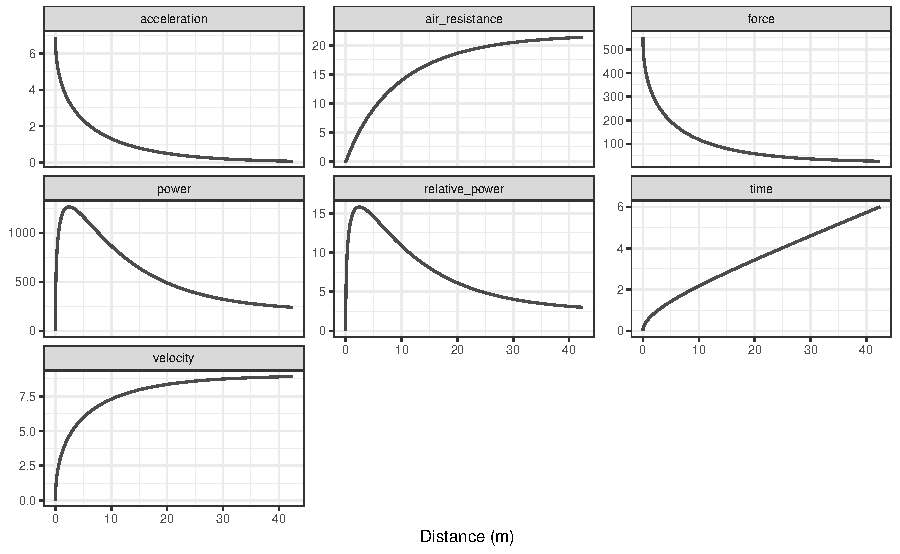
\includegraphics[width=1\linewidth]{paper_files/figure-latex/unnamed-chunk-7-1} \end{center}

\end{CodeChunk}

\hypertarget{utility-functions}{%
\subsubsection{Utility functions}\label{utility-functions}}

Another valuable addition for sport scientists and coaches is the ability to determine the distances and times where 90\% of maximum sprinting speed is reached, or where peak power is within 90\% range. To identify these values, \pkg{shorts} package comes with \texttt{find\_} family of functions:

\begin{CodeChunk}
\begin{CodeInput}
R> # Finds distance where 90% of maximum sprinting speed is reached
R> find_velocity_critical_distance(
+   MSS = m1$parameters$MSS,
+   TAU = m1$parameters$TAU,
+   percent = 0.9
+ )
\end{CodeInput}
\begin{CodeOutput}
#> [1] 16.5
\end{CodeOutput}
\begin{CodeInput}
R> 
R> # Finds maximal power and distance (this time using air resistance)
R> find_max_power_distance(
+   MSS = m1$parameters$MSS,
+   TAU = m1$parameters$TAU,
+   # Additional parameters forwarded to get_air_resistance
+   # Otherwise, defaults are used
+   bodymass = 80,
+   bodyheight = 1.85,
+   barometric_pressure = 780,
+   air_temperature = 20,
+   wind_velocity = 0.5
+ )
\end{CodeInput}
\begin{CodeOutput}
#> $max_power
#> [1] 1264
#> 
#> $distance
#> [1] 2.46
\end{CodeOutput}
\begin{CodeInput}
R> 
R> # Finds distance over 90% power range
R> find_power_critical_distance(
+   MSS = m1$parameters$MSS,
+   TAU = m1$parameters$TAU,
+   # Additional parameters forwarded to get_air_resistance
+   # Otherwise, defaults are used
+   bodymass = 80,
+   bodyheight = 1.85,
+   barometric_pressure = 780,
+   air_temperature = 20,
+   wind_velocity = 0.5
+ )
\end{CodeInput}
\begin{CodeOutput}
#> $lower
#> [1] 0.959
#> 
#> $upper
#> [1] 5.44
\end{CodeOutput}
\end{CodeChunk}

\hypertarget{mixed-effects-model}{%
\subsubsection{Mixed-effects model}\label{mixed-effects-model}}

Sprint performance is often evaluated with a group of athletes (e.g., soccer club) representing a single strata of interest. Sports scientists can estimate individual profiles, or utilize mixed-effects models. To perform mixed-effects models in \pkg{shorts} for split times, one can use \texttt{mixed\_model\_using\_splits} function. To demonstrate this functionality, we load the \texttt{split\_times} dataset provided in the \pkg{shorts} package:

\begin{CodeChunk}
\begin{CodeInput}
R> data(split_times)
R> 
R> # Mixed model
R> m2 <- mixed_model_using_splits(
+   data = split_times,
+   distance = "distance",
+   time = "time",
+   athlete = "athlete",
+ 
+   # Select random effects
+   # Default is MSS and TAU
+   random = MSS + TAU ~ 1
+ )
R> 
R> m2
\end{CodeInput}
\begin{CodeOutput}
#> Estimated fixed model parameters
#> --------------------------------
#>                 MSS                 TAU                 MAC 
#>               8.065               0.655              12.309 
#>                PMAX     time_correction distance_correction 
#>              24.818               0.000               0.000 
#> 
#> Estimated random model parameters
#> ----------------------------------
#>     athlete  MSS   TAU  MAC PMAX time_correction distance_correction
#> 1     James 9.69 0.847 11.4 27.7               0                   0
#> 2       Jim 7.83 0.505 15.5 30.4               0                   0
#> 3      John 7.78 0.727 10.7 20.8               0                   0
#> 4 Kimberley 8.57 0.802 10.7 22.9               0                   0
#> 5  Samantha 6.45 0.395 16.3 26.4               0                   0
#> 
#> Model fit estimators
#> --------------------
#>       RSE R_squared    minErr    maxErr maxAbsErr      RMSE       MAE 
#>    0.0260    0.9998   -0.0293    0.0496    0.0496    0.0214    0.0172 
#>      MAPE 
#>    0.9019
\end{CodeOutput}
\end{CodeChunk}

Additional information about mixed-effects model performed using the \texttt{nlme} package \citep{R-nlme} can be obtained using \texttt{summary}:

\begin{CodeChunk}
\begin{CodeInput}
R> summary(m2)
\end{CodeInput}
\begin{CodeOutput}
#> Nonlinear mixed-effects model fit by maximum likelihood
#>   Model: corrected_time ~ TAU * I(LambertW::W(-exp(1)^(-distance/(MSS *      TAU) - 1))) + distance/MSS + TAU 
#>  Data: train 
#>     AIC   BIC logLik
#>   -75.1 -66.7   43.5
#> 
#> Random effects:
#>  Formula: list(MSS ~ 1, TAU ~ 1)
#>  Level: athlete
#>  Structure: General positive-definite, Log-Cholesky parametrization
#>          StdDev Corr 
#> MSS      1.066  MSS  
#> TAU      0.178  0.877
#> Residual 0.026       
#> 
#> Fixed effects: MSS + TAU ~ 1 
#>     Value Std.Error DF t-value p-value
#> MSS  8.06     0.495 24   16.30       0
#> TAU  0.66     0.084 24    7.82       0
#>  Correlation: 
#>     MSS  
#> TAU 0.874
#> 
#> Standardized Within-Group Residuals:
#>    Min     Q1    Med     Q3    Max 
#> -1.909 -0.605  0.154  0.523  1.129 
#> 
#> Number of Observations: 30
#> Number of Groups: 5
\end{CodeOutput}
\end{CodeChunk}

The following figure contains kinematics for all athletes in \texttt{split\_times} dataset. Please note that power calculation takes default parameters for each individual:

\begin{CodeChunk}
\begin{CodeInput}
R> df <- predict_kinematics(m2, max_time = 10)
R> 
R> df <- pivot_longer(df, cols = c(-1, -3))
R> 
R> ggplot(
+   filter(df, distance < 40),
+   aes(x = distance, y = value, group = athlete, color = athlete)
+ ) +
+   theme_bw(8) +
+   facet_wrap(~name, scales = "free_y") +
+   geom_line(alpha = 0.7) +
+   ylab(NULL) +
+   xlab("Distance (m)") +
+   theme(
+     legend.position = "top",
+     legend.title = element_blank())
\end{CodeInput}


\begin{center}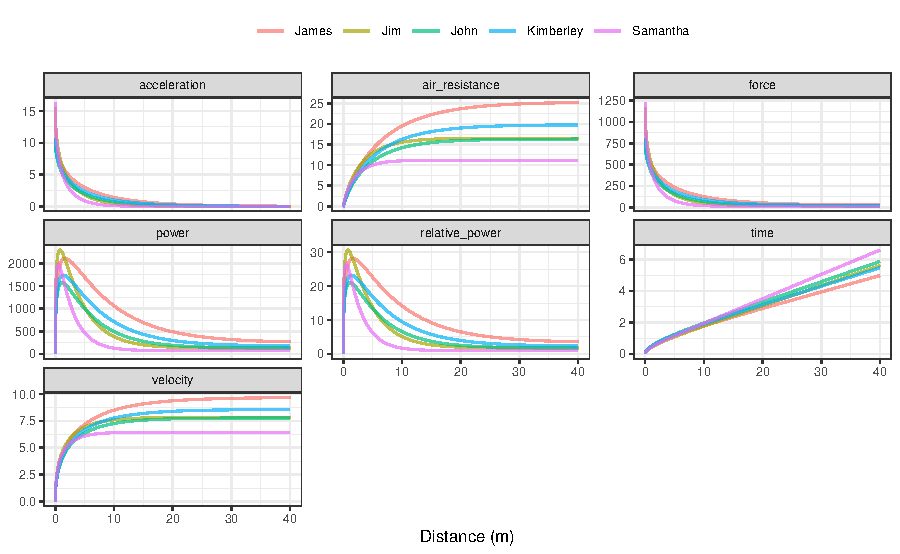
\includegraphics[width=1\linewidth]{paper_files/figure-latex/unnamed-chunk-11-1} \end{center}

\end{CodeChunk}

\hypertarget{estimating-short-sprint-parameters-using-radar-gun}{%
\subsection{Estimating short sprint parameters using radar gun}\label{estimating-short-sprint-parameters-using-radar-gun}}

Estimation of the short sprint profile using radar gun data takes time as predictor and velocity as the outcome variable. Thus equation \eqref{eq:velocity-time} is used to estimate MSS and TAU.

Let's consider the same example of an athlete with MSS equal to 9\(ms^-1\), TAU equal to 1.3, and MAC equal to 6.92\(ms^-2\) performing 40m sprint with velocity estimated using radar run (in this case with 1Hz sampling rate).

\begin{CodeChunk}
\begin{CodeInput}
R> sprint_time <- seq(0, 6, 1)
R> 
R> sprint_velocity <- c(0.00, 4.83, 7.07, 8.10, 8.59, 8.81, 8.91)
R> 
R> m3 <- model_using_radar(
+   velocity = sprint_velocity,
+   time = sprint_time
+ )
R> 
R> m3
\end{CodeInput}
\begin{CodeOutput}
#> Estimated model parameters
#> --------------------------
#>                 MSS                 TAU                 MAC 
#>                9.00                1.30                6.92 
#>                PMAX     time_correction distance_correction 
#>               15.58                0.00                0.00 
#> 
#> Model fit estimators
#> --------------------
#>       RSE R_squared    minErr    maxErr maxAbsErr      RMSE       MAE 
#>   0.00327   1.00000  -0.00406   0.00532   0.00532   0.00276   0.00207 
#>      MAPE 
#>       NaN
\end{CodeOutput}
\end{CodeChunk}

Both split and radar gun models allow the use of \emph{weighted} non-linear regression. For example, we can give more weight to shorter distance or faster velocities. Weighted non-linear regression is performed by setting \texttt{weights} parameter:

\begin{CodeChunk}
\begin{CodeInput}
R> m3_weighted <- model_using_radar(
+   velocity = sprint_velocity,
+   time = sprint_time,
+   weights = 1 / (sprint_velocity + 1)
+ )
R> 
R> m3_weighted
\end{CodeInput}
\begin{CodeOutput}
#> Estimated model parameters
#> --------------------------
#>                 MSS                 TAU                 MAC 
#>                9.00                1.30                6.92 
#>                PMAX     time_correction distance_correction 
#>               15.58                0.00                0.00 
#> 
#> Model fit estimators
#> --------------------
#>       RSE R_squared    minErr    maxErr maxAbsErr      RMSE       MAE 
#>   0.00108   1.00000  -0.00406   0.00534   0.00534   0.00276   0.00206 
#>      MAPE 
#>       NaN
\end{CodeOutput}
\end{CodeChunk}

\hypertarget{mixed-effects-model-1}{%
\subsubsection{Mixed-effects model}\label{mixed-effects-model-1}}

Mixed-effects model using radar data is done using \texttt{mixed\_model\_using\_radar} function. To perform mixed model, let's load data that comes with \pkg{shorts} package.

\begin{CodeChunk}
\begin{CodeInput}
R> data("radar_gun_data")
R> 
R> m4 <- mixed_model_using_radar(
+   radar_gun_data,
+   time = "time",
+   velocity = "velocity",
+   athlete = "athlete"
+ )
R> 
R> m4
\end{CodeInput}
\begin{CodeOutput}
#> Estimated fixed model parameters
#> --------------------------------
#>                 MSS                 TAU                 MAC 
#>                8.30                1.01                8.24 
#>                PMAX     time_correction distance_correction 
#>               17.09                0.00                0.00 
#> 
#> Estimated random model parameters
#> ----------------------------------
#>     athlete   MSS   TAU  MAC PMAX time_correction distance_correction
#> 1     James 10.00 1.111 9.00 22.5               0                   0
#> 2       Jim  8.00 0.889 9.00 18.0               0                   0
#> 3      John  8.00 1.069 7.48 15.0               0                   0
#> 4 Kimberley  9.01 1.286 7.01 15.8               0                   0
#> 5  Samantha  6.50 0.685 9.50 15.4               0                   0
#> 
#> Model fit estimators
#> --------------------
#>       RSE R_squared    minErr    maxErr maxAbsErr      RMSE       MAE 
#>    0.0516    0.9994   -0.2191    0.1983    0.2191    0.0516    0.0395 
#>      MAPE 
#>       NaN
\end{CodeOutput}
\end{CodeChunk}

\hypertarget{problems-with-estimation}{%
\section{Problems with estimation}\label{problems-with-estimation}}

There is a challenge when collecting sprint data that could have a substantial impact on modeled outcomes. To ensure accurate parameter outcomes, the initial force production must be synced with start time \citep{haugenPowerForceVelocityProfilingSprinting2020, haugenSprintMechanicalVariables2019}. Below we describe this challenge when using radar guns or timing gates and suggest potential solutions within the \pkg{shorts} package.

\hypertarget{problems-with-time-sync-with-radar-gun}{%
\subsection{Problems with time sync with radar gun}\label{problems-with-time-sync-with-radar-gun}}

One source of error in the modeled estimation using a radar gun is the time synchronization. In theory, synchronization is ideal when a sprint is initiated at \(t=0\) (i.e., \(v(t=0) = 0\)). In practice, this is often not the case. Let's use our athlete and add and deduct 0.5s to simulate an error in synchronization and its effect on estimated MSS and TAU (Figure \ref{fig:radar-gun-sync}).

The following three models estimate MSS and TAU from the three datasets:

\begin{CodeChunk}
\begin{CodeInput}
R> # Without synchronization issues
R> m5 <- model_using_radar(
+   velocity = df$velocity,
+   time = df$`true time`
+ )
R> 
R> # With time added
R> m6 <- model_using_radar(
+   velocity = df$velocity,
+   time = df$`0.5s added`
+ )
R> 
R> # With time deducted
R> m7 <- model_using_radar(
+   velocity = df$velocity,
+   time = df$`0.5s deducted`
+ )
R> 
R> rbind(
+   data.frame(
+     model = "True time",
+     t(coef(m5))
+   ),
+   data.frame(
+     model = "Added 0.5s time",
+     t(coef(m6))
+   ),
+   data.frame(
+     model = "Deducted 0.5s time",
+     t(coef(m7))
+   )
+ )
\end{CodeInput}
\begin{CodeOutput}
#>                model   MSS  TAU  MAC PMAX time_correction
#> 1          True time  9.00 1.30 6.92 15.6               0
#> 2    Added 0.5s time  9.91 2.34 4.23 10.5               0
#> 3 Deducted 0.5s time 10.08 1.86 5.43 13.7               0
#>   distance_correction
#> 1                   0
#> 2                   0
#> 3                   0
\end{CodeOutput}
\end{CodeChunk}

As can be seen from the example, TAU is affected by an error in synchronization of time with velocity. The potential solution incorporated into the \pkg{shorts} package involves estimation of the \emph{time correction} parameter using the following equation:

\begin{equation}
  v(t) = MSS \times (1 - e^{-\frac{t + time \; correction}{TAU}}) \label{eq:velocity-time-correction}
\end{equation}

This model is incorporated in the \texttt{model\_using\_radar\_with\_time\_correction} function:

\begin{CodeChunk}
\begin{CodeInput}
R> # With time added
R> m8 <- model_using_radar_with_time_correction(
+   velocity = df$velocity,
+   time = df$`0.5s added`
+ )
R> coef(m8)
\end{CodeInput}
\begin{CodeOutput}
#>                 MSS                 TAU                 MAC 
#>                9.00                1.30                6.92 
#>                PMAX     time_correction distance_correction 
#>               15.58               -0.50                0.00
\end{CodeOutput}
\begin{CodeInput}
R> 
R> # With time deducted
R> m9 <- model_using_radar_with_time_correction(
+   velocity = df$velocity,
+   time = df$`0.5s deducted`
+ )
R> coef(m9)
\end{CodeInput}
\begin{CodeOutput}
#>                 MSS                 TAU                 MAC 
#>                9.00                1.30                6.92 
#>                PMAX     time_correction distance_correction 
#>               15.58                0.50                0.00
\end{CodeOutput}
\end{CodeChunk}

When using \texttt{predict\_} family of functions, one can provide estimated time correction to get predictions at original time scale.

\begin{CodeChunk}
\begin{CodeInput}
R> # Using the true time
R> predict_velocity_at_time(
+   time = df$`true time`,
+   MSS = m5$parameters$MSS,
+   TAU = m5$parameters$TAU
+ )
\end{CodeInput}
\begin{CodeOutput}
#> [1] 0.00 4.83 7.07 8.11 8.59 8.81 8.91
\end{CodeOutput}
\begin{CodeInput}
R> 
R> # Using time with sync issues
R> predict_velocity_at_time(
+   time = df$`0.5s added`,
+   MSS = m8$parameters$MSS,
+   TAU = m8$parameters$TAU,
+   time_correction = m8$parameters$time_correction
+ )
\end{CodeInput}
\begin{CodeOutput}
#> [1] 7.82e-05 4.83e+00 7.07e+00 8.11e+00 8.59e+00 8.81e+00 8.91e+00
\end{CodeOutput}
\end{CodeChunk}

\hypertarget{mixed-model-approach}{%
\subsubsection{Mixed-model approach}\label{mixed-model-approach}}

When it comes to mixed-model approach, time correction can be modeled as a fixed effect or random effect using the \texttt{mixed\_model\_using\_radar\_with\_time\_correction} function.

\begin{CodeChunk}
\begin{CodeInput}
R> # Adding 0.5s to radar_gun_data
R> radar_gun_data$time <- radar_gun_data$time + 0.5
R> 
R> # Mixed model with time correction being fixed effect
R> m10 <- mixed_model_using_radar_with_time_correction(
+   radar_gun_data,
+   time = "time",
+   velocity = "velocity",
+   athlete = "athlete",
+   random = MSS + TAU ~ 1
+ )
R> 
R> m10
\end{CodeInput}
\begin{CodeOutput}
#> Estimated fixed model parameters
#> --------------------------------
#>                 MSS                 TAU                 MAC 
#>                8.30                1.01                8.24 
#>                PMAX     time_correction distance_correction 
#>               17.10               -0.50                0.00 
#> 
#> Estimated random model parameters
#> ----------------------------------
#>     athlete   MSS   TAU  MAC PMAX time_correction distance_correction
#> 1     James 10.00 1.111 9.00 22.5            -0.5                   0
#> 2       Jim  8.00 0.889 9.00 18.0            -0.5                   0
#> 3      John  8.00 1.069 7.48 15.0            -0.5                   0
#> 4 Kimberley  9.01 1.285 7.01 15.8            -0.5                   0
#> 5  Samantha  6.50 0.685 9.50 15.4            -0.5                   0
#> 
#> Model fit estimators
#> --------------------
#>       RSE R_squared    minErr    maxErr maxAbsErr      RMSE       MAE 
#>    0.0516    0.9994   -0.2190    0.1983    0.2190    0.0516    0.0395 
#>      MAPE 
#>       Inf
\end{CodeOutput}
\begin{CodeInput}
R> 
R> # Mixed model with time correction being random effect
R> m11 <- mixed_model_using_radar_with_time_correction(
+   radar_gun_data,
+   time = "time",
+   velocity = "velocity",
+   athlete = "athlete",
+   random = MSS + TAU + time_correction ~ 1
+ )
R> 
R> m11
\end{CodeInput}
\begin{CodeOutput}
#> Estimated fixed model parameters
#> --------------------------------
#>                 MSS                 TAU                 MAC 
#>                8.30                1.01                8.24 
#>                PMAX     time_correction distance_correction 
#>               17.10               -0.50                0.00 
#> 
#> Estimated random model parameters
#> ----------------------------------
#>     athlete   MSS   TAU  MAC PMAX time_correction distance_correction
#> 1     James 10.00 1.110 9.00 22.5            -0.5                   0
#> 2       Jim  8.00 0.889 9.00 18.0            -0.5                   0
#> 3      John  8.00 1.069 7.48 15.0            -0.5                   0
#> 4 Kimberley  9.01 1.285 7.01 15.8            -0.5                   0
#> 5  Samantha  6.50 0.685 9.50 15.4            -0.5                   0
#> 
#> Model fit estimators
#> --------------------
#>       RSE R_squared    minErr    maxErr maxAbsErr      RMSE       MAE 
#>    0.0516    0.9994   -0.2188    0.1982    0.2188    0.0516    0.0395 
#>      MAPE 
#>       Inf
\end{CodeOutput}
\end{CodeChunk}

\hypertarget{problems-at-the-start-when-using-split-times}{%
\subsection{Problems at the start when using split times}\label{problems-at-the-start-when-using-split-times}}

Let's imagine we have two twin brothers with same short sprint characteristics: MSS equal to 9\(ms^-1\), TAU equal to 1.3, and MAC equal to 6.92\(ms^-2\). Let's call them John and Jack. They both perform 40m sprint using timing gates set at 5, 10, 20, 30, and 40m. The initial timing gate at the start (i.e., \(d=0m\)) serves to activate the timing system (i.e., when they cross the beam).

John represents the \emph{theoretical model}, in which we assume that the initial force production and the timing initiation are perfectly synchronized. Jack, on the other hand, represents a \emph{practical model}, and decides to move slightly behind the initial timing gate (i.e.~for 0.5m) and use body rocking to initiate the sprint start. In other words, Jack is using a \emph{flying start}, a common scenario when testing field sports athletes. Let's see how their sprint outcomes differ.

\begin{CodeChunk}
\begin{CodeInput}
R> MSS <- 9
R> TAU <- 1.3
R> MAC <- MSS / TAU
R> 
R> split_times <- tibble(
+   distance = c(5, 10, 20, 30, 40),
+   john_time = predict_time_at_distance(distance, MSS, TAU),
+ 
+   # Jack's performance
+   jack_distance = distance + 0.5,
+   jack_true_time = predict_time_at_distance(jack_distance, MSS, TAU),
+   time_05m = predict_time_at_distance(0.5, MSS, TAU),
+   jack_time = jack_true_time - time_05m
+ )
R> 
R> split_times
\end{CodeInput}
\begin{CodeOutput}
#> # A tibble: 5 x 6
#>   distance john_time jack_distance jack_true_time time_05m jack_time
#>      <dbl>  <I<dbl>>         <dbl>       <I<dbl>> <I<dbl>>  <I<dbl>>
#> 1        5      1.42           5.5           1.50    0.400      1.10
#> 2       10      2.17          10.5           2.23    0.400      1.83
#> 3       20      3.43          20.5           3.49    0.400      3.09
#> 4       30      4.60          30.5           4.65    0.400      4.25
#> 5       40      5.73          40.5           5.78    0.400      5.39
\end{CodeOutput}
\end{CodeChunk}

And here is a graphical representation of the sprint splits:

\begin{CodeChunk}
\begin{CodeInput}
R> plot_df <- split_times %>%
+   select(distance, john_time, jack_time) %>%
+   rename(John = john_time, Jack = jack_time) %>%
+   pivot_longer(cols = -1, names_to = "athlete", values_to = "time") %>%
+   mutate(distance = factor(distance))
R> 
R> ggplot(
+   plot_df,
+   aes(x = distance, y = time, color = athlete, group = athlete)
+ ) +
+   theme_bw(8) +
+   geom_point() +
+   geom_line() +
+   xlab("Distance (m)") +
+   ylab("Time (s)") +
+   theme(
+     legend.title = element_blank(), 
+     legend.position = "top")
\end{CodeInput}


\begin{center}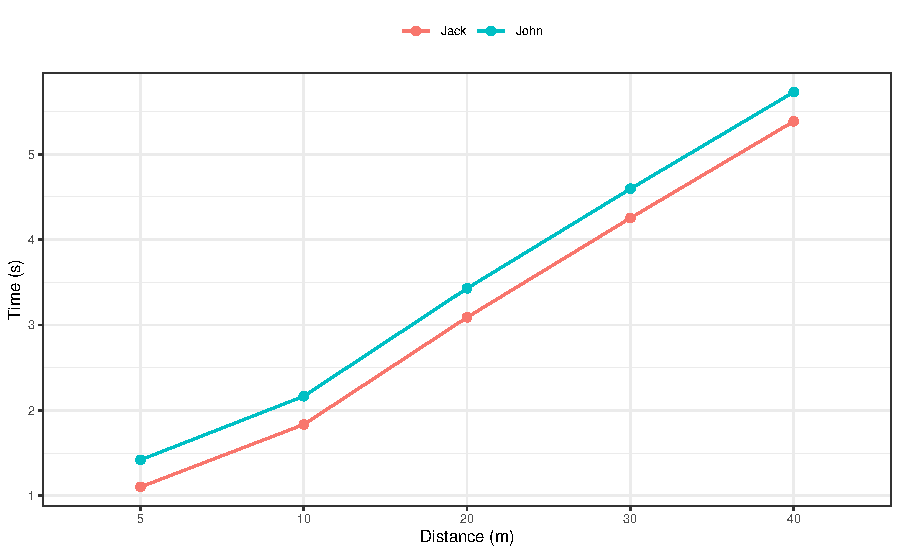
\includegraphics[width=1\linewidth]{paper_files/figure-latex/unnamed-chunk-20-1} \end{center}

\end{CodeChunk}

Using the following code, we can see the differences in estimated MSS and TAU parameters:

\begin{CodeChunk}
\begin{CodeInput}
R> # Since this is a perfect simulation and stats::nls will complain
R> # we need to add very small noise, or measurement error to the times
R> set.seed(1667)
R> rand_noise <- rnorm(nrow(split_times), 0, 10^-5)
R> split_times$john_time <- split_times$john_time + rand_noise
R> split_times$jack_time <- split_times$jack_time + rand_noise
R> 
R> john_profile <- model_using_splits(
+   distance = split_times$distance,
+   time = split_times$john_time
+ )
R> 
R> jack_profile <- model_using_splits(
+   distance = split_times$distance,
+   time = split_times$jack_time
+ )
R> 
R> sprint_parameters <- rbind(
+   unlist(john_profile$parameters),
+   unlist(jack_profile$parameters)
+ )
R> 
R> rownames(sprint_parameters) <- c("John", "Jack")
R> 
R> sprint_parameters
\end{CodeInput}
\begin{CodeOutput}
#>       MSS   TAU   MAC PMAX time_correction distance_correction
#> John 9.00 1.300  6.92 15.6               0                   0
#> Jack 8.49 0.704 12.06 25.6               0                   0
\end{CodeOutput}
\end{CodeChunk}

As can be seen from the results, a flying start yields biased estimates, particularly for the TAU, MAC and PMAX.

Below is a simulation sprint with 5, 10, 20, 30, 40, and 50m splits, with MSS and MAC varying from 6 to 9 (\(ms^-1\) and \(ms^-2\) respectively), and flying start distance varying from 0 to 1m.

\begin{CodeChunk}
\begin{CodeInput}
R> sim_df <- expand.grid(
+   MSS = c(6, 7, 8, 9),
+   MAC = c(6, 7, 8, 9),
+   flying_start_distance = c(
+     seq(0, 0.001, length.out = 20),
+     seq(0.001, 0.01, length.out = 20),
+     seq(0.01, 0.1, length.out = 20),
+     seq(0.1, 1, length.out = 20)
+   ),
+   distance = c(5, 10, 20, 30, 40, 50)
+ )
R> 
R> sim_df <- sim_df %>%
+   mutate(
+     TAU = MSS / MAC,
+     PMAX = MSS * MAC / 4,
+     true_distance = distance + flying_start_distance,
+     true_time = predict_time_at_distance(true_distance, MSS, TAU),
+     stolen_time = predict_time_at_distance(flying_start_distance, MSS, TAU),
+     time = true_time - stolen_time
+   )
R> 
R> # Add small noise to allow model fit
R> set.seed(1667)
R> rand_noise <- rnorm(nrow(sim_df), 0, 10^-4)
R> sim_df$time <- sim_df$time + rand_noise
\end{CodeInput}
\end{CodeChunk}

Now when we have a simulation dataset, we can check the model estimates and predictions, given the flying start distance:

\begin{CodeChunk}
\begin{CodeInput}
R> # Prediction wrapper
R> pred_wrapper <- function(data) {
+   model <- model_using_splits(
+     distance = data$distance,
+     time = data$time
+   )
+ 
+   params <- data.frame(t(unlist(model$parameters)))
+ 
+   predicted_time <- predict_time_at_distance(
+     distance = data$distance,
+     MSS = model$parameters$MSS,
+     TAU = model$parameters$TAU
+   )
+ 
+   colnames(params) <- c(
+     "est_MSS", "est_TAU", "est_MAC", "est_PMAX",
+     "est_time_correction", "est_distance_correction"
+   )
+ 
+   cbind(
+     data,
+     params,
+     data.frame(predicted_time = as.numeric(predicted_time))
+   )
+ }
R> 
R> # estimated parameters and predicted time
R> model_df <- sim_df %>%
+   group_by(MSS, TAU, flying_start_distance) %>%
+   do(pred_wrapper(.)) %>%
+   ungroup()
R> 
R> # Prediction residuals
R> model_df$residuals <- model_df$predicted_time - model_df$time
\end{CodeInput}
\end{CodeChunk}

The following image demonstrates the effect of flying start distance on estimated MSS:

\begin{CodeChunk}
\begin{CodeInput}
R> # Estimates plot
R> df <- model_df %>%
+   group_by(MSS, TAU, flying_start_distance) %>%
+   slice(1) %>%
+   mutate(
+     MSS_string = paste("MSS =", MSS),
+     TAU_string = paste("TAU =", TAU),
+     MAC_string = paste("MAC = ", round(MAC, 2)),
+     PMAX_string = paste("PMAX = ", round(PMAX, 2))
+   )
R> 
R> # MSS
R> ggplot(
+   df,
+   aes(x = flying_start_distance, y = est_MSS, color = MAC_string)
+ ) +
+   theme_bw(8) +
+   geom_line(alpha = 0.7) +
+   facet_wrap(~MSS_string, scales = "free_y") +
+   xlab("Flying start distance (m)") +
+   ylab("estimated MSS (m/s)") +
+   theme(
+     legend.title = element_blank(), 
+     legend.position = "top")
\end{CodeInput}


\begin{center}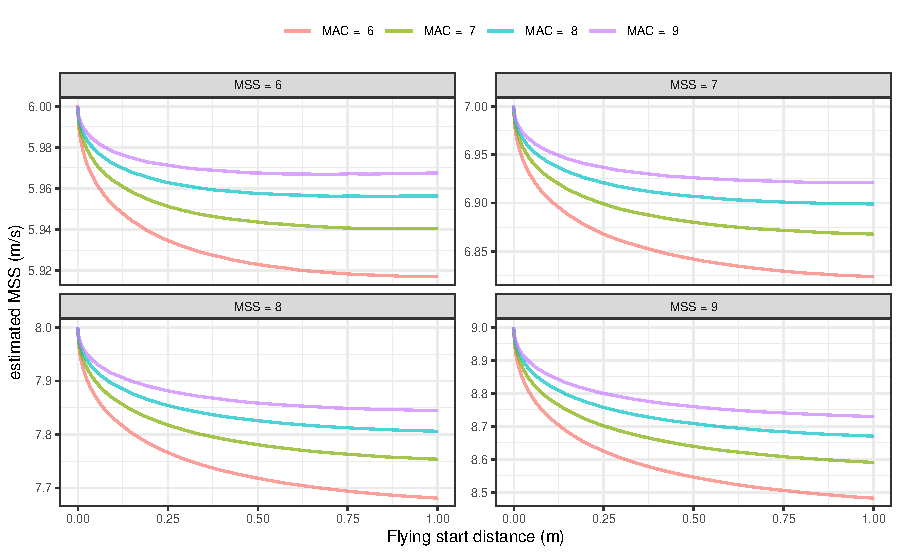
\includegraphics[width=1\linewidth]{paper_files/figure-latex/unnamed-chunk-24-1} \end{center}

\end{CodeChunk}

As can be seen from the image, MSS is underestimated as flying start distance increases. The following image demonstrates the effect of flying start distance on estimated MAC:

\begin{CodeChunk}
\begin{CodeInput}
R> # MAC
R> ggplot(
+   df,
+   aes(x = flying_start_distance, y = est_MAC, color = MSS_string)
+ ) +
+   theme_bw(8) +
+   geom_line(alpha = 0.7) +
+   facet_wrap(~MAC_string, scales = "free_y") +
+   xlab("Flying start distance (m)") +
+   ylab("estimated MAC (m/s/s)") +
+   theme(
+     legend.title = element_blank(), 
+     legend.position = "top")
\end{CodeInput}


\begin{center}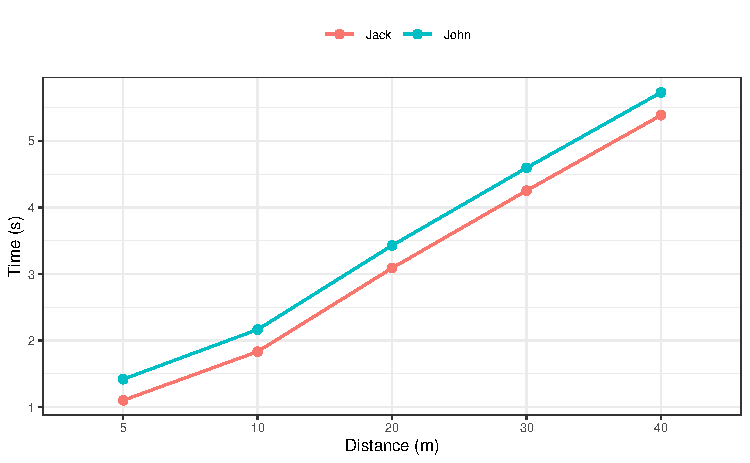
\includegraphics[width=1\linewidth]{paper_files/figure-latex/unnamed-chunk-25-1} \end{center}

\end{CodeChunk}

MAC (and also TAU) are highly affected by the flying start distance, and from the figure we can notice that MAC is overestimated as flying start distance increases.

And finally, the following image demonstrates the effect of flying start distance on estimated PMAX:

\begin{CodeChunk}
\begin{CodeInput}
R> # PMAX
R> ggplot(
+   df,
+   aes(x = flying_start_distance, y = est_PMAX, color = MSS_string)
+ ) +
+   theme_bw(8) +
+   geom_line(alpha = 0.7) +
+   facet_wrap(~MAC_string, scales = "free_y") +
+   xlab("Flying start distance (m)") +
+   ylab("estimated PMAX (W/kg)") +
+   theme(
+     legend.title = element_blank(), 
+     legend.position = "top")
\end{CodeInput}


\begin{center}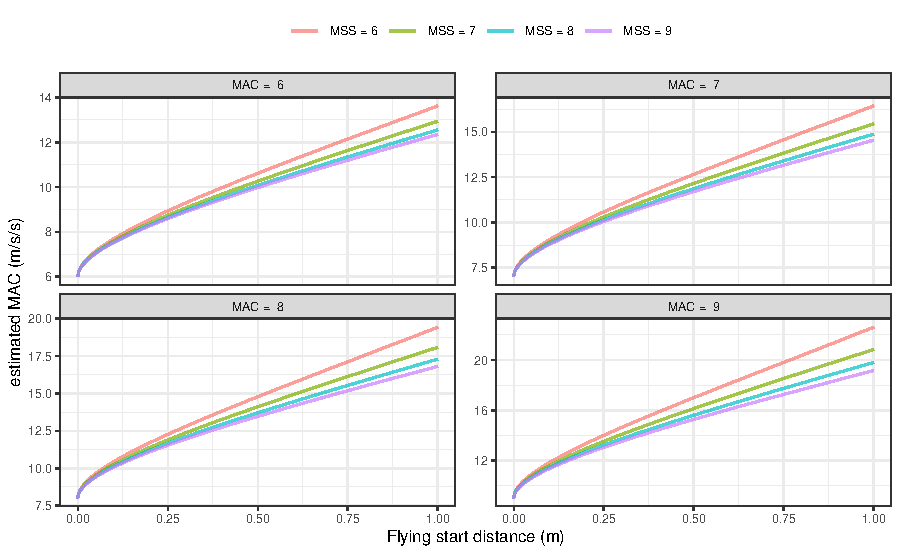
\includegraphics[width=1\linewidth]{paper_files/figure-latex/unnamed-chunk-26-1} \end{center}

\end{CodeChunk}

Estimated PMAX is also overestimated as flying start distance increases.

Model residuals are also affected by flying start distance. The shape of residuals distribution depends on number and splits utilized (e.g., 10, 20, 30, 40m versus 5, 15, 30m), but here we can see the effect of the flying start distance on the model residuals per split distance utilized in our simulation:

\begin{CodeChunk}
\begin{CodeInput}
R> # Residuals
R> model_df <- model_df %>%
+   mutate(
+     MSS_string = paste("MSS =", MSS),
+     TAU_string = paste("TAU =", TAU),
+     MAC_string = paste("MAC = ", round(MAC, 2)),
+     PMAX_string = paste("PMAX = ", round(PMAX, 2)),
+     group = paste(MSS, MAC, flying_start_distance)
+   )
R> 
R> ggplot(
+   model_df,
+   aes(y = residuals, x = distance, color = flying_start_distance, group = group)
+ ) +
+   theme_bw(8) +
+   geom_line(alpha = 0.3) +
+   facet_grid(MSS_string ~ MAC_string) +
+   geom_hline(yintercept = 0, linetype = "dashed") +
+   scale_color_gradientn(colours = terrain.colors(5, rev = FALSE)) +
+   xlab("Distance (m)") +
+   ylab("Predicted time - observed time (s)") +
+   theme(legend.position = "top") + 
+   labs(color = "Flying start distance")
\end{CodeInput}


\begin{center}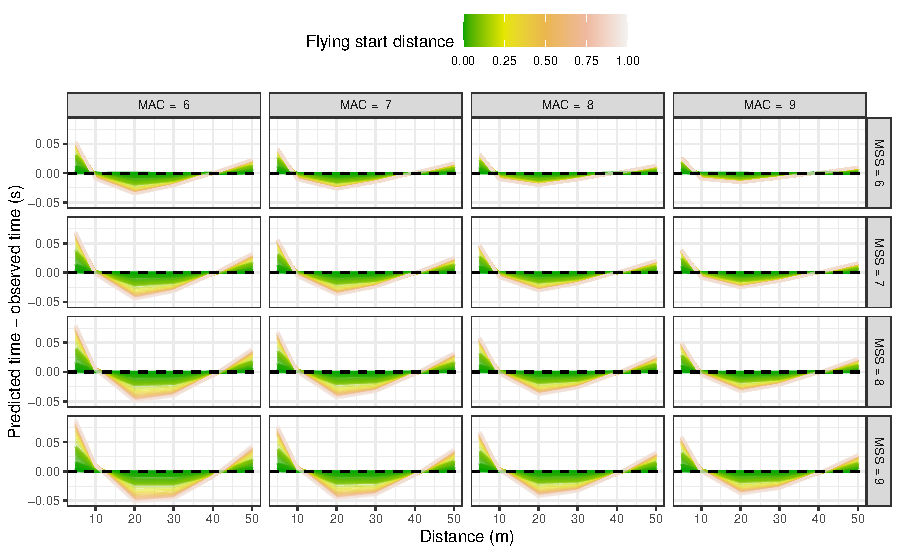
\includegraphics[width=1\linewidth]{paper_files/figure-latex/unnamed-chunk-27-1} \end{center}

\end{CodeChunk}

If we merge individual facets (i.e., combinations of MSS and MAC), we can get simpler images conveying issues with residuals when there is a flying start:

\begin{CodeChunk}
\begin{CodeInput}
R> ggplot(
+   model_df,
+   aes(y = residuals, x = distance, color = flying_start_distance, group = group)
+ ) +
+   theme_bw(8) +
+   geom_line(alpha = 0.3) +
+   geom_hline(yintercept = 0, linetype = "dashed") +
+   scale_color_gradientn(colours = terrain.colors(5, rev = FALSE)) +
+   xlab("Distance (m)") +
+   ylab("Predicted time - observed time (s)") +
+   theme(legend.position = "top") + 
+   labs(color = "Flying start distance")
\end{CodeInput}


\begin{center}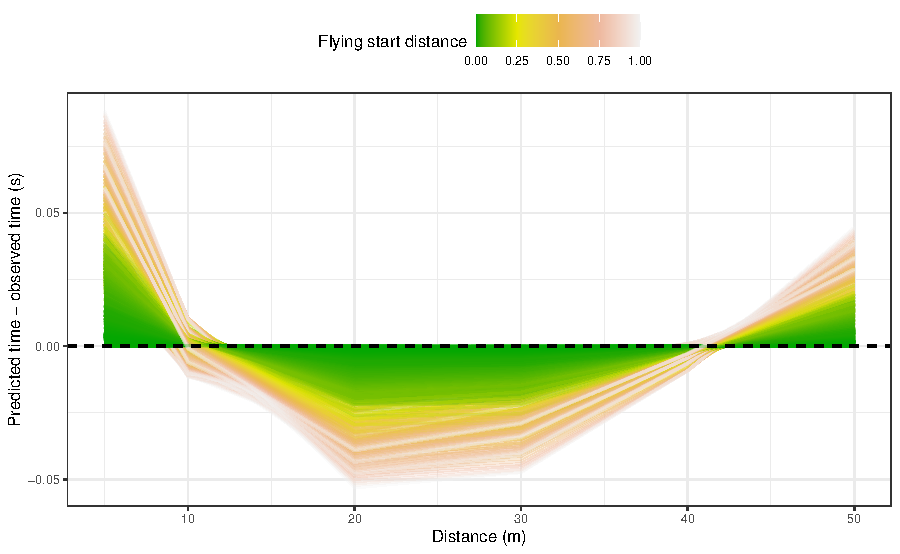
\includegraphics[width=1\linewidth]{paper_files/figure-latex/unnamed-chunk-28-1} \end{center}

\end{CodeChunk}

Clearly, any type of flying start where there is a difference between initial force production and start time can result in biased parameters and predictions. Since maximal sprint speed is difficult to improve, the effects of start inconsistencies can mask effects of the training intervention. It is thus crucial to standardize the start when testing and implementing the following techniques when using the \pkg{shorts} package.

\hypertarget{how-to-overcome-missing-the-initial-force-production-when-using-timing-gates}{%
\subsubsection{How to overcome missing the initial force production when using timing gates?}\label{how-to-overcome-missing-the-initial-force-production-when-using-timing-gates}}

A potential solution is to use a correction factor - the recommendation in the literature is +0.5sec \citep{haugenSprintMechanicalProperties2020, haugenSprintMechanicalVariables2019}. Interestingly, the average difference between using timing gates and a block start for 40 m sprint time was 0.27 sec \citep{haugenDifferenceStartImpact2012}. So, while a timing correction factor is warranted to avoid subsequent errors in estimates of kinetic variables (e.g., overestimate power), a correction factor that is too large will have the opposite effect (e.g., underestimate power).

When implementing \emph{time correction}, equation \eqref{eq:time-distance} becomes:

\begin{equation}
  t(d) = TAU \times W(-e^{\frac{-d}{MSS \times TAU}} - 1) + \frac{d}{MSS} + TAU - time \; correction \label{eq:time-correction}
\end{equation}

Rather than providing \emph{apriori} time correction from the literature, \pkg{shorts} package provides an estimation of this parameter from the data provided, together with MSS and TAU. To estimate time correction, we use \texttt{model\_using\_splits\_with\_time\_correction} function. Here is how we can estimate Jack parameters using either provided time correction (e.g., +0.3 and +0.5s) or estimated time correction:

\begin{CodeChunk}
\begin{CodeInput}
R> jack_profile_fixed_time_short <- model_using_splits(
+   distance = split_times$distance,
+   time = split_times$jack_time,
+   time_correction = 0.3
+ )
R> 
R> jack_profile_fixed_time_long <- model_using_splits(
+   distance = split_times$distance,
+   time = split_times$jack_time,
+   time_correction = 0.5
+ )
R> 
R> jack_profile_time_estimated <- model_using_splits_with_time_correction(
+   distance = split_times$distance,
+   time = split_times$jack_time
+ )
R> 
R> jack_parameters <- rbind(
+   unlist(john_profile$parameters),
+   unlist(jack_profile$parameters),
+   unlist(jack_profile_fixed_time_short$parameters),
+   unlist(jack_profile_fixed_time_long$parameters),
+   unlist(jack_profile_time_estimated$parameters)
+ )
R> 
R> rownames(jack_parameters) <- c(
+   "John",
+   "Jack - No corrections",
+   "Jack - Fixed time correction (+0.3s)",
+   "Jack - Fixed time correction (+0.5s)",
+   "Jack - Estimated time correction"
+ )
R> 
R> jack_parameters
\end{CodeInput}
\begin{CodeOutput}
#>                                       MSS   TAU   MAC PMAX
#> John                                 9.00 1.300  6.92 15.6
#> Jack - No corrections                8.49 0.704 12.06 25.6
#> Jack - Fixed time correction (+0.3s) 9.00 1.251  7.19 16.2
#> Jack - Fixed time correction (+0.5s) 9.62 1.770  5.43 13.1
#> Jack - Estimated time correction     8.96 1.216  7.37 16.5
#>                                      time_correction
#> John                                           0.000
#> Jack - No corrections                          0.000
#> Jack - Fixed time correction (+0.3s)           0.300
#> Jack - Fixed time correction (+0.5s)           0.500
#> Jack - Estimated time correction               0.284
#>                                      distance_correction
#> John                                                   0
#> Jack - No corrections                                  0
#> Jack - Fixed time correction (+0.3s)                   0
#> Jack - Fixed time correction (+0.5s)                   0
#> Jack - Estimated time correction                       0
\end{CodeOutput}
\end{CodeChunk}

In Jack's case, both +0.3s fixed time correction and time correction estimation yield parameters closer to John's (i.e.~true parameters).

Another model definition, which is a novel approach implemented in the \pkg{shorts} packages, is to utilize \emph{distance correction}, besides time correction. Thus, equation \eqref{eq:time-distance} becomes:

\begin{equation}
  t(d) = TAU \times W(-e^{\frac{-d + distance \; correction}{MSS \times TAU}} - 1) + \frac{d + distance \; correction}{MSS} + TAU - time \; correction \label{eq:distance-correction}
\end{equation}

This model is implemented in \texttt{model\_using\_splits\_with\_corrections} function. Below are the model estimates:

\begin{CodeChunk}
\begin{CodeInput}
R> jack_profile_distance_correction <- model_using_splits_with_corrections(
+   distance = split_times$distance,
+   time = split_times$jack_time
+ )
R> 
R> jack_parameters <- rbind(
+   unlist(john_profile$parameters),
+   unlist(jack_profile$parameters),
+   unlist(jack_profile_fixed_time_short$parameters),
+   unlist(jack_profile_fixed_time_long$parameters),
+   unlist(jack_profile_time_estimated$parameters),
+   unlist(jack_profile_distance_correction$parameters)
+ )
R> 
R> rownames(jack_parameters) <- c(
+   "John",
+   "Jack - No corrections",
+   "Jack - Fixed time correction (+0.3s)",
+   "Jack - Fixed time correction (+0.5s)",
+   "Jack - Estimated time correction",
+   "Jack - Estimated distance correction"
+ )
R> 
R> jack_parameters
\end{CodeInput}
\begin{CodeOutput}
#>                                       MSS   TAU   MAC PMAX
#> John                                 9.00 1.300  6.92 15.6
#> Jack - No corrections                8.49 0.704 12.06 25.6
#> Jack - Fixed time correction (+0.3s) 9.00 1.251  7.19 16.2
#> Jack - Fixed time correction (+0.5s) 9.62 1.770  5.43 13.1
#> Jack - Estimated time correction     8.96 1.216  7.37 16.5
#> Jack - Estimated distance correction 9.00 1.301  6.92 15.6
#>                                      time_correction
#> John                                           0.000
#> Jack - No corrections                          0.000
#> Jack - Fixed time correction (+0.3s)           0.300
#> Jack - Fixed time correction (+0.5s)           0.500
#> Jack - Estimated time correction               0.284
#> Jack - Estimated distance correction           0.400
#>                                      distance_correction
#> John                                               0.000
#> Jack - No corrections                              0.000
#> Jack - Fixed time correction (+0.3s)               0.000
#> Jack - Fixed time correction (+0.5s)               0.000
#> Jack - Estimated time correction                   0.000
#> Jack - Estimated distance correction               0.503
\end{CodeOutput}
\end{CodeChunk}

As can be seen from the results, adding distance correction results in correctly estimating Jack's sprint parameters. There are a few issues with this model definition. Besides being novel and still not validated with actual data, distance correction model has four parameters to estimate, which implies that at least five sprint splits are needed. This imposes practical limitations, since acquiring six timing gate (one for the start and five for splits) might be practically troublesome.

We will get back to these issues later, but we can examine how these models perform using simulated data with varying flying start distance. The following code contains the wrapper that performs all four models (no correction, fixed time correction, estimated time correction, and estimated time and distance correction):

\begin{CodeChunk}
\begin{CodeInput}
R> pred_wrapper <- function(data) {
+   no_correction <- model_using_splits(
+     distance = data$distance,
+     time = data$time
+   )
+ 
+   fixed_correction_short <- model_using_splits(
+     distance = data$distance,
+     time = data$time,
+     time_correction = 0.3
+   )
+ 
+   fixed_correction_long <- model_using_splits(
+     distance = data$distance,
+     time = data$time,
+     time_correction = 0.5
+   )
+ 
+   time_correction <- model_using_splits_with_time_correction(
+     distance = data$distance,
+     time = data$time,
+     control = nls.control(tol = 1)
+   )
+ 
+   time_dist_correction <- model_using_splits_with_corrections(
+     distance = data$distance,
+     time = data$time,
+     control = nls.control(tol = 1)
+   )
+ 
+ 
+   params <- rbind(
+     data.frame(
+       model = "No correction",
+       t(unlist(no_correction$parameters))
+     ),
+     data.frame(
+       model = "Fixed correction +0.3s",
+       t(unlist(fixed_correction_short$parameters))
+     ),
+     data.frame(
+       model = "Fixed correction +0.5s",
+       t(unlist(fixed_correction_long$parameters))
+     ),
+     data.frame(
+       model = "Time correction",
+       t(unlist(time_correction$parameters))
+     ),
+     data.frame(
+       model = "Time and distance correction",
+       t(unlist(time_dist_correction$parameters))
+     )
+   )
+ 
+   colnames(params) <- c(
+     "model", "est_MSS", "est_TAU", "est_MAC", "est_PMAX",
+     "est_time_correction", "est_distance_correction"
+   )
+ 
+   df <- expand_grid(
+     data,
+     params
+   )
+ 
+   df$predicted_time <- predict_time_at_distance(
+     distance = df$distance,
+     MSS = df$est_MSS,
+     TAU = df$est_TAU,
+     time_correction = df$est_time_correction,
+     distance_correction = df$est_distance_correction
+   )
+ 
+   df$residuals <- df$predicted_time - df$time
+   return(df)
+ }
R> 
R> # estimated parameters and predicted time
R> model_df <- sim_df %>%
+   group_by(MSS, TAU, flying_start_distance) %>%
+   do(pred_wrapper(.)) %>%
+   ungroup()
\end{CodeInput}
\end{CodeChunk}

As can be seen from the next figure, the estimated time correction model estimates MSS almost perfectly, while the estimated time and distance correction model estimates MSS perfectly.

\begin{CodeChunk}
\begin{CodeInput}
R> model_df$model <- factor(
+   model_df$model,
+   levels = c(
+     "No correction",
+     "Fixed correction +0.3s",
+     "Fixed correction +0.5s",
+     "Time correction",
+     "Time and distance correction"
+   )
+ )
R> # Estimates plot
R> df <- model_df %>%
+   group_by(MSS, TAU, flying_start_distance, model) %>%
+   slice(1) %>%
+   mutate(
+     MSS_string = paste("MSS =", MSS),
+     TAU_string = paste("TAU =", TAU),
+     MAC_string = paste("MAC = ", round(MAC, 2)),
+     PMAX_string = paste("PMAX = ", round(PMAX, 2))
+   )
R> 
R> # MSS
R> ggplot(
+   df,
+   aes(x = flying_start_distance, y = est_MSS, color = model)
+ ) +
+   theme_bw(8) +
+   geom_line(alpha = 0.7) +
+   facet_grid(MSS_string ~ MAC_string, scales = "free_y") +
+   xlab("Flying start distance (m)") +
+   ylab("estimated MSS (m/s)") +
+   theme(
+     legend.title = element_blank(),
+     legend.position = "top")
\end{CodeInput}


\begin{center}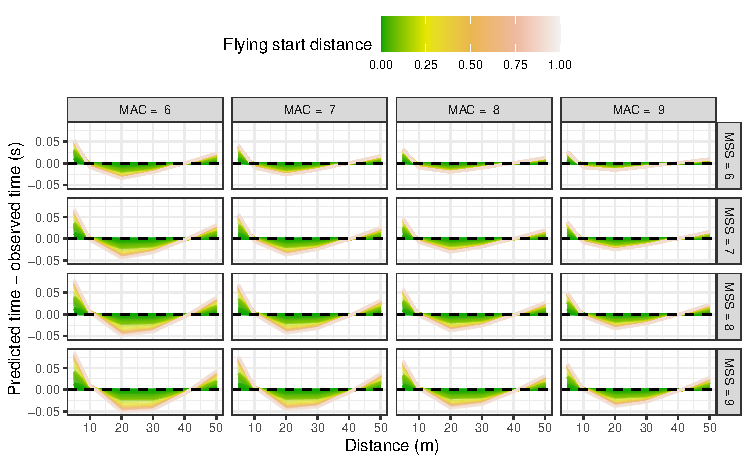
\includegraphics[width=1\linewidth]{paper_files/figure-latex/unnamed-chunk-32-1} \end{center}

\end{CodeChunk}

Similar outcomes are observed for the MAC parameter. The time and distance corrections model performs perfectly, while the time correction model performs almost as good.

\begin{CodeChunk}
\begin{CodeInput}
R> # MAC
R> ggplot(
+   df,
+   aes(x = flying_start_distance, y = est_MAC, color = model)
+ ) +
+   theme_bw(8) +
+   geom_line(alpha = 0.7) +
+   facet_grid(MAC_string ~ MSS_string, scales = "free_y") +
+   xlab("Flying start distance (m)") +
+   ylab("estimated MAC (m/s/s)") +
+   theme(
+     legend.title = element_blank(),
+     legend.position = "top")
\end{CodeInput}


\begin{center}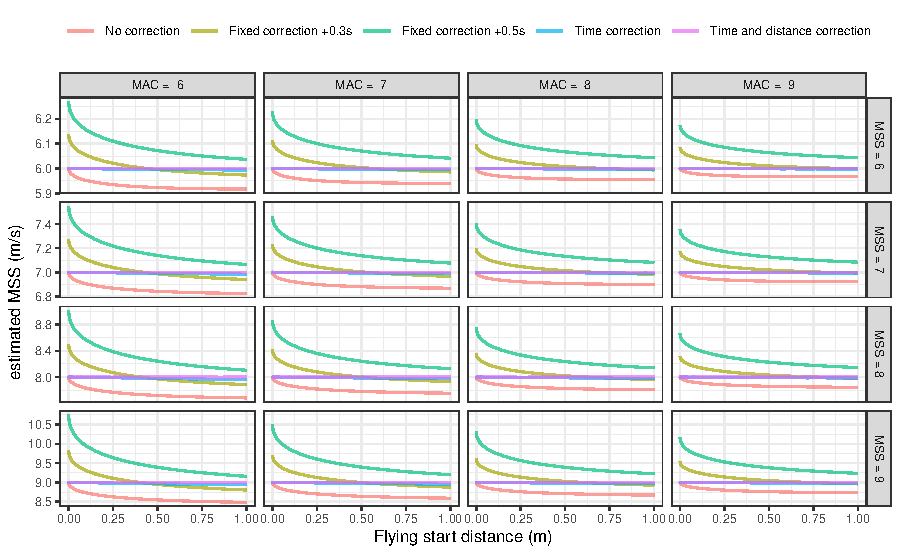
\includegraphics[width=1\linewidth]{paper_files/figure-latex/unnamed-chunk-33-1} \end{center}

\end{CodeChunk}

PMAX demonstrates the same properties as MSS and MAC.

\begin{CodeChunk}
\begin{CodeInput}
R> # PMAX
R> ggplot(
+   df,
+   aes(x = flying_start_distance, y = est_PMAX, color = model)
+ ) +
+   theme_bw(8) +
+   geom_line(alpha = 0.7) +
+   facet_grid(MAC_string ~ MSS_string, scales = "free_y") +
+   xlab("Flying start distance (m)") +
+   ylab("estimated PMAX (W/kg)") +
+   theme(
+     legend.title = element_blank(),
+     legend.position = "top")
\end{CodeInput}


\begin{center}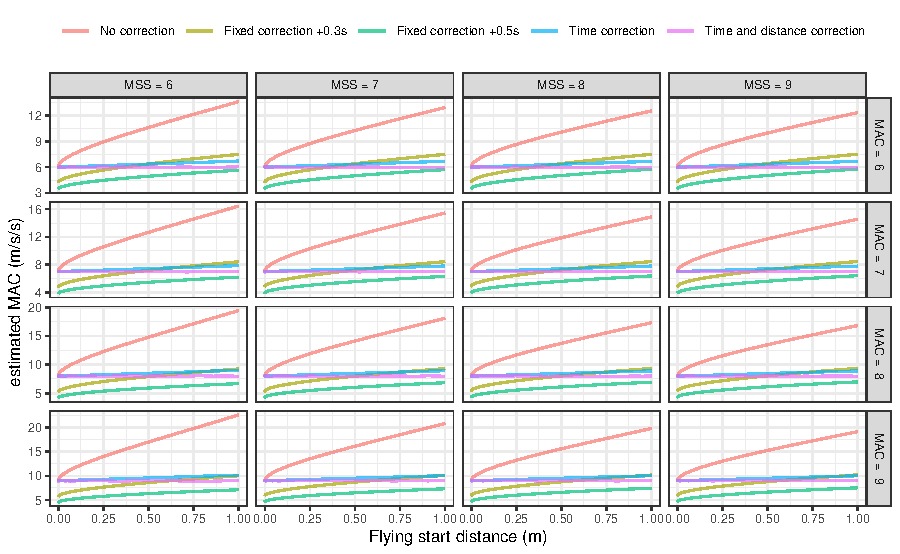
\includegraphics[width=1\linewidth]{paper_files/figure-latex/unnamed-chunk-34-1} \end{center}

\end{CodeChunk}

The following figure depicts estimated time correction, and as can be seen, only the time and distance correction model estimated the time correction correctly (i.e., the \emph{stolen time}; indicated by the dashed line on the figure).

\begin{CodeChunk}
\begin{CodeInput}
R> # time_correction
R> ggplot(
+   df,
+   aes(x = flying_start_distance, y = est_time_correction, color = model)
+ ) +
+   theme_bw(8) +
+   geom_line(alpha = 0.7) +
+   geom_line(aes(y = stolen_time), color = "black", linetype = "dashed") +
+   facet_grid(MAC_string ~ MSS_string, scales = "free_y") +
+   xlab("Flying start distance (m)") +
+   ylab("estimated time correction (s)")  +
+   theme(
+     legend.title = element_blank(),
+     legend.position = "top")
\end{CodeInput}


\begin{center}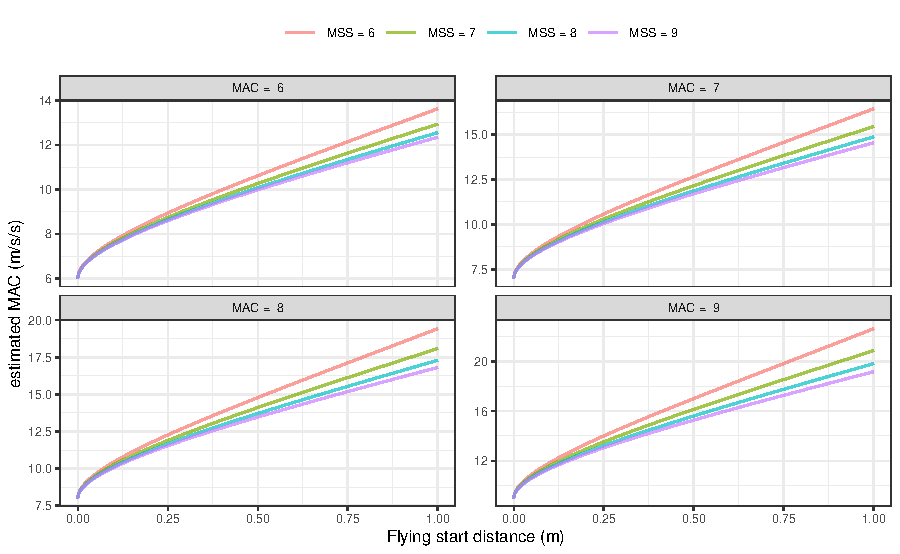
\includegraphics[width=1\linewidth]{paper_files/figure-latex/unnamed-chunk-35-1} \end{center}

\end{CodeChunk}

The following figure depicts estimated distance correction, and same as with the time correction, only the time and distance correction model estimated the distance correction correctly (i.e., flying start distance; indicated by the dashed line on the figure, which represents \emph{identity line} since flying start distance is already on the x-axis).

\begin{CodeChunk}
\begin{CodeInput}
R> # distance_correction
R> ggplot(
+   df,
+   aes(x = flying_start_distance, y = est_distance_correction, color = model)
+ ) +
+   theme_bw(8) +
+   geom_line(alpha = 0.7) +
+   geom_abline(slope = 1, color = "black", linetype = "dashed") +
+   facet_grid(MAC_string ~ MSS_string, scales = "free_y") +
+   xlab("Flying start distance (m)") +
+   ylab("estimated distance correction (m)") +
+   theme(
+     legend.title = element_blank(),
+     legend.position = "top")
\end{CodeInput}


\begin{center}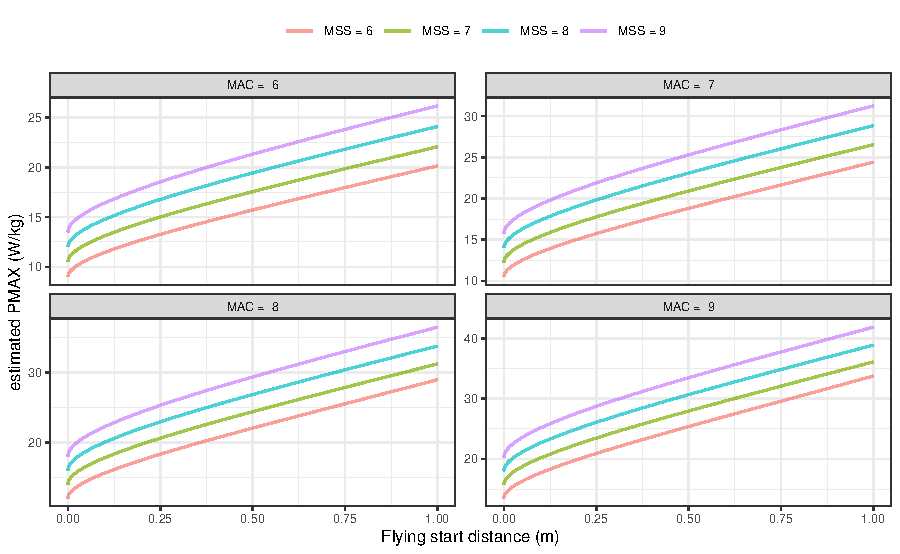
\includegraphics[width=1\linewidth]{paper_files/figure-latex/unnamed-chunk-36-1} \end{center}

\end{CodeChunk}

The following figure depicts model residuals against the distance, and as can be seen, time correction and time and distance correction models performs much better than no correction and fixed correction models:

\begin{CodeChunk}
\begin{CodeInput}
R> # Residuals
R> model_df <- model_df %>%
+   mutate(
+     MSS_string = paste("MSS =", MSS),
+     TAU_string = paste("TAU =", TAU),
+     MAC_string = paste("MAC = ", round(MAC, 2)),
+     PMAX_string = paste("PMAX = ", round(PMAX, 2)),
+     group = paste(MSS, MAC, flying_start_distance)
+   )
R> 
R> ggplot(
+   model_df,
+   aes(y = residuals, x = distance, color = flying_start_distance, group = group)
+ ) +
+   theme_bw(8) +
+   geom_line(alpha = 0.3) +
+   facet_wrap(~model) +
+   geom_hline(yintercept = 0, linetype = "dashed") +
+   scale_color_gradientn(colours = terrain.colors(5, rev = FALSE)) +
+   xlab("Distance (m)") +
+   ylab("Predicted time - observed time (s)") +
+   theme(legend.position = "top") + 
+   labs(color = "Flying start distance")
\end{CodeInput}


\begin{center}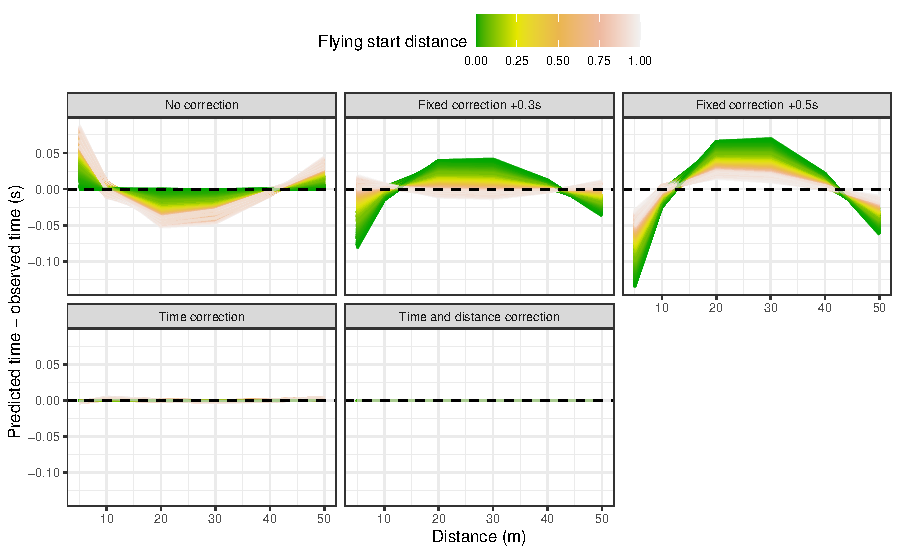
\includegraphics[width=1\linewidth]{paper_files/figure-latex/unnamed-chunk-37-1} \end{center}

\end{CodeChunk}

The outcomes from the simulation data clearly demonstrates that the time correction and time and distance correction models represent sound improvements in parameter estimation and model fit compared to no corrections model and fixed correction model when attempting to overcome the flying start issues. Since the time correction model is simpler and requires three parameters to be estimated, it might be practically more useful than the time and distance correction model, which requires four parameters estimation and thus more than five timing gates and sprint splits.

Time correction and time and distance corrections are also implemented in the mixed-models using \texttt{mixed\_model\_using\_splits\_with\_time\_correction} and \texttt{mixed\_model\_using\_splits\_with\_corrections}. We will showcase their use at the end of this article.

\hypertarget{simulation-of-additional-starting-issues}{%
\subsubsection{Simulation of additional starting issues}\label{simulation-of-additional-starting-issues}}

Starting behind the initial timing gate represent only one issue (i.e.~flying start). In this section, we simulate one more issue to check the sensitivity of the presented models to other (less common) perturbations when performing field testing.

One issue that might happen with timing gates is triggering the timing system before the sprint is initiated (e.g., by cutting the beam with an arm swing prematurely). This is very similar to the situation when timing starts on a signal (i.e., gun during 100m sprint race) and there is \emph{reaction time} (RT) involved. Both of these scenarios represent \emph{time lag} that is added to the split times. Below we simulate the effect of this time lag on model estimates and predictions.

\begin{CodeChunk}
\begin{CodeInput}
R> sim_df <- expand.grid(
+   MSS = c(6, 7, 8, 9),
+   MAC = c(6, 7, 8, 9),
+   time_lag = seq(0, 0.5, length.out = 50),
+   distance = c(5, 10, 20, 30, 40, 50)
+ )
R> 
R> sim_df <- sim_df %>%
+   mutate(
+     TAU = MSS / MAC,
+     PMAX = MSS * MAC / 4,
+     true_time = predict_time_at_distance(distance, MSS, TAU),
+     time = true_time + time_lag
+   )
R> 
R> # Add small noise to allow model fit
R> set.seed(1667)
R> rand_noise <- rnorm(nrow(sim_df), 0, 10^-4)
R> sim_df$time <- sim_df$time + rand_noise
\end{CodeInput}
\end{CodeChunk}

\begin{CodeChunk}
\begin{CodeInput}
R> # estimated parameters and predicted time
R> model_df <- sim_df %>%
+   group_by(MSS, TAU, time_lag) %>%
+   do(pred_wrapper(.)) %>%
+   ungroup()
\end{CodeInput}
\end{CodeChunk}

From the figure below it can be seen that time lag affects estimated MSS for the the model without correction and fixed correction model. Time correction and time and distance corrections models correctly estimated MSS.

\begin{CodeChunk}
\begin{CodeInput}
R> model_df$model <- factor(
+   model_df$model,
+   levels = c(
+     "No correction",
+     "Fixed correction +0.3s",
+     "Fixed correction +0.5s",
+     "Time correction",
+     "Time and distance correction"
+   )
+ )
R> # Estimates plot
R> df <- model_df %>%
+   group_by(MSS, TAU, time_lag, model) %>%
+   slice(1) %>%
+   mutate(
+     MSS_string = paste("MSS =", MSS),
+     TAU_string = paste("TAU =", TAU),
+     MAC_string = paste("MAC = ", round(MAC, 2)),
+     PMAX_string = paste("PMAX = ", round(PMAX, 2))
+   )
R> 
R> # MSS
R> ggplot(df, aes(x = time_lag, y = est_MSS, color = model)) +
+   theme_bw(8) +
+   geom_line(alpha = 0.7) +
+   facet_grid(MSS_string ~ MAC_string, scales = "free_y") +
+   xlab("Time lag (s)") +
+   ylab("estimated MSS (m/s)") +
+   theme(
+     legend.title = element_blank(),
+     legend.position = "top")
\end{CodeInput}


\begin{center}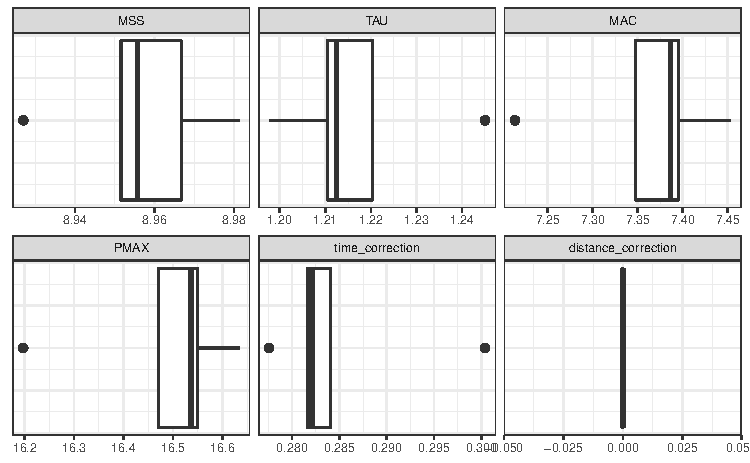
\includegraphics[width=1\linewidth]{paper_files/figure-latex/unnamed-chunk-40-1} \end{center}

\end{CodeChunk}

From the figure below it can be seen that time lag affects estimated MAC for the the model without correction and fixed correction models. Time correction and time and distance corrections model correctly estimated MAC.

\begin{CodeChunk}
\begin{CodeInput}
R> # MAC
R> ggplot(df, aes(x = time_lag, y = est_MAC, color = model)) +
+   theme_bw(8) +
+   geom_line(alpha = 0.7) +
+   facet_grid(MAC_string ~ MSS_string, scales = "free_y") +
+   xlab("Time lag (s)") +
+   ylab("estimated MAC (m/s/s)") +
+   theme(
+     legend.title = element_blank(),
+     legend.position = "top")
\end{CodeInput}


\begin{center}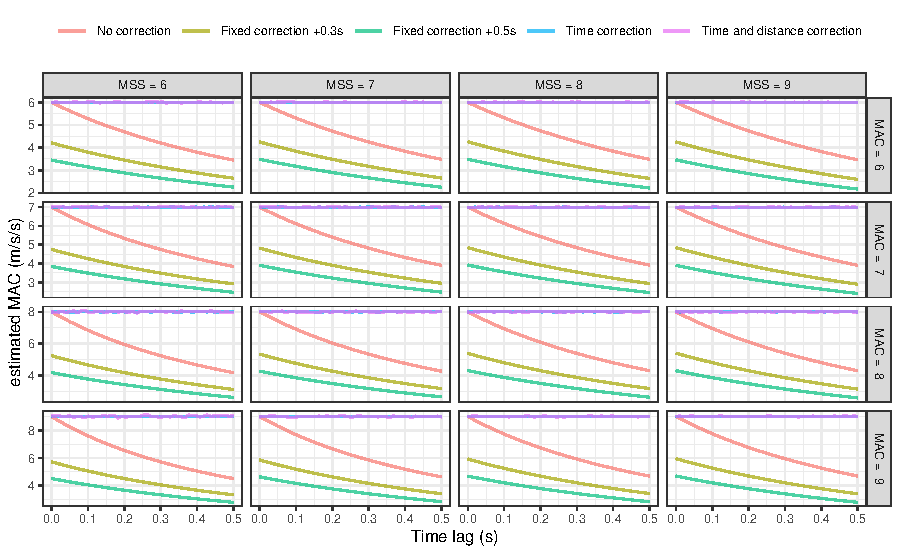
\includegraphics[width=1\linewidth]{paper_files/figure-latex/unnamed-chunk-41-1} \end{center}

\end{CodeChunk}

The figure below depicts correctly identified time lag (i.e.~using time correction parameter) using time correction and time and distance corrections models.

\begin{CodeChunk}
\begin{CodeInput}
R> # time_correction
R> ggplot(
+   df,
+   aes(x = time_lag, y = est_time_correction, color = model)
+ ) +
+   theme_bw(8) +
+   geom_line(alpha = 0.7) +
+   geom_abline(slope = -1, color = "black", linetype = "dashed") +
+   facet_grid(MAC_string ~ MSS_string, scales = "free_y") +
+   xlab("Time lag (s)") +
+   ylab("estimated time correction (s)") +
+   theme(
+     legend.title = element_blank(),
+     legend.position = "top")
\end{CodeInput}


\begin{center}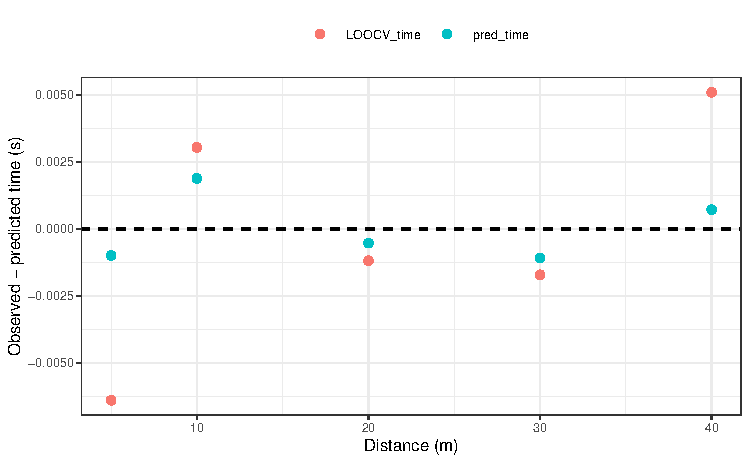
\includegraphics[width=1\linewidth]{paper_files/figure-latex/unnamed-chunk-42-1} \end{center}

\end{CodeChunk}

The next figure depicts estimated distance correction for the time and distance correction model. The estimated distance correction parameters looks jumpy due to random noise that we have to added to allow model fit.

\begin{CodeChunk}
\begin{CodeInput}
R> # distance_correction
R> ggplot(
+   df,
+   aes(x = time_lag, y = est_distance_correction, color = model)
+ ) +
+   theme_bw(8) +
+   geom_line(alpha = 0.7) +
+   facet_grid(MAC_string ~ MSS_string, scales = "free_y") +
+   xlab("Time lag (s)") +
+   ylab("estimated distance correction (m)") +
+   theme(
+     legend.title = element_blank(),
+     legend.position = "top")
\end{CodeInput}


\begin{center}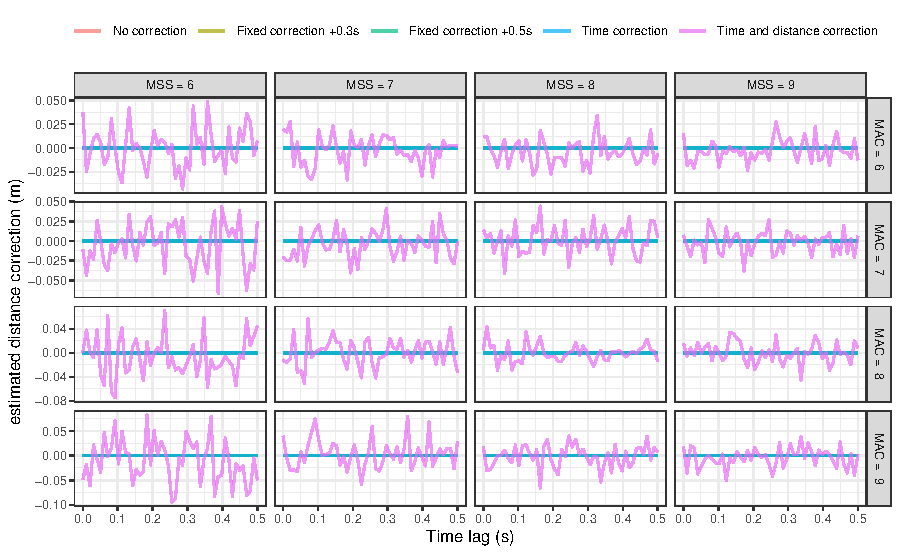
\includegraphics[width=1\linewidth]{paper_files/figure-latex/unnamed-chunk-43-1} \end{center}

\end{CodeChunk}

The following figure depicts residuals (i.e., predicted time minus observed time).

\begin{CodeChunk}
\begin{CodeInput}
R> # Residuals
R> model_df <- model_df %>%
+   mutate(
+     MSS_string = paste("MSS =", MSS),
+     TAU_string = paste("TAU =", TAU),
+     MAC_string = paste("MAC = ", round(MAC, 2)),
+     PMAX_string = paste("PMAX = ", round(PMAX, 2)),
+     group = paste(MSS, MAC, time_lag)
+   )
R> 
R> ggplot(
+   model_df,
+   aes(y = residuals, x = distance, color = time_lag, group = group)
+ ) +
+   theme_bw(8) +
+   geom_line(alpha = 0.3) +
+   facet_wrap(~model) +
+   geom_hline(yintercept = 0, linetype = "dashed") +
+   scale_color_gradientn(colours = terrain.colors(5, rev = FALSE)) +
+   xlab("Distance (m)") +
+   ylab("Predicted time - observed time (s)")  +
+   theme(legend.position = "top") + 
+   labs(color = "Time lag")
\end{CodeInput}


\begin{center}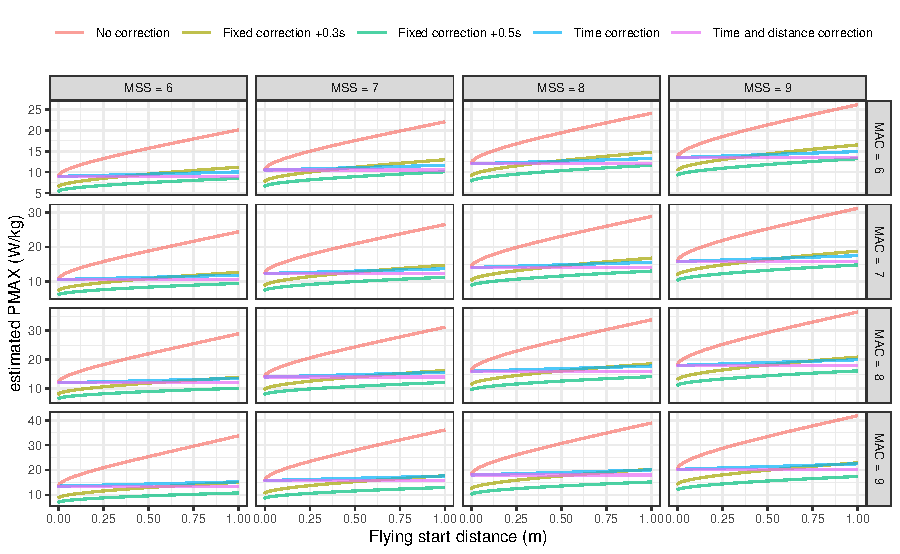
\includegraphics[width=1\linewidth]{paper_files/figure-latex/unnamed-chunk-44-1} \end{center}

\end{CodeChunk}

There are few other starting issues worth mentioning. For example, if the initial timing gate has a time delay (i.e., once triggered, there is a time delay before the timing starts). In this case, time lag is a negative number since it reduces the split times. Another common issue with timing gates in the practical field settings is the bad measurement of the distance and thus bad positions of the timing gates.

The number and distances of the timing gates can also affect the precision of the estimated sprint parameters \citep{haugenPowerForceVelocityProfilingSprinting2020, haugenDifferenceStartImpact2012}.

In field testing, multiple starting issues can be present. For example, one might have a bad position of the initial gate, athlete might be moved back but also manage to trigger the gate before the start commence. More elaborate simulation is beyond the scope of the current paper.

\hypertarget{leave-one-out-cross-validation}{%
\section{Leave-one-out Cross-Validation}\label{leave-one-out-cross-validation}}

To estimate parameter stability, model over-fitting, and performance on the unseen data, \pkg{shorts} model function comes with implemented \emph{leave-one-out cross validation} (LOOCV) \citep{jamesIntroductionStatisticalLearning2017, jovanovicBmbstatsBootstrapMagnitudebased2020, kuhnAppliedPredictiveModeling2018}. LOOCV involves a simple, yet powerful procedure, of removing each observation, rebuilding the model, and making predictions for that removed observation. This process is repeated for each observations in the model dataset. LOOCV allows one to check estimated parameters stability, and model performance on the unseen data.

Let's perform LOOCV using Jack's data and the time correction model:

\begin{CodeChunk}
\begin{CodeInput}
R> jack_LOOCV <- model_using_splits_with_time_correction(
+   distance = split_times$distance,
+   time = split_times$jack_time,
+   LOOCV = TRUE
+ )
R> 
R> jack_LOOCV
\end{CodeInput}
\begin{CodeOutput}
#> Estimated model parameters
#> --------------------------
#>                 MSS                 TAU                 MAC 
#>               8.958               1.216               7.367 
#>                PMAX     time_correction distance_correction 
#>              16.499               0.284               0.000 
#> 
#> Model fit estimators
#> --------------------
#>       RSE R_squared    minErr    maxErr maxAbsErr      RMSE       MAE 
#>   0.00181   1.00000  -0.00109   0.00189   0.00189   0.00114   0.00104 
#>      MAPE 
#>   0.04981 
#> 
#> 
#> Leave-One-Out Cross-Validation
#> ------------------------------
#> Parameters:
#>    MSS  TAU  MAC PMAX time_correction distance_correction
#> 1 8.98 1.25 7.21 16.2           0.300                   0
#> 2 8.97 1.22 7.35 16.5           0.284                   0
#> 3 8.95 1.21 7.40 16.5           0.282                   0
#> 4 8.96 1.21 7.39 16.5           0.282                   0
#> 5 8.93 1.20 7.45 16.6           0.278                   0
#> 
#> Model fit:
#>       RSE R_squared    minErr    maxErr maxAbsErr      RMSE       MAE 
#>        NA   1.00000  -0.00639   0.00510   0.00639   0.00401   0.00349 
#>      MAPE 
#>   0.18387
\end{CodeOutput}
\end{CodeChunk}

The model print output provides training dataset estimates and model performance, as well as LOOCV estimates and model performance.

Next we plot estimated parameters across LOOCV folds:

\begin{CodeChunk}
\begin{CodeInput}
R> df <- jack_LOOCV$LOOCV$parameters
R> 
R> df <- pivot_longer(df, cols = 1:6, names_to = "parameter")
R> 
R> df$parameter <- factor(
+   df$parameter,
+   levels = c(
+     "MSS",
+     "TAU",
+     "MAC",
+     "PMAX",
+     "time_correction",
+     "distance_correction"
+   )
+ )
R> 
R> ggplot(df, aes(x = value)) +
+   theme_bw(8) +
+   geom_boxplot() +
+   facet_wrap(~parameter, scales = "free_x") +
+   xlab(NULL) +
+   ylab(NULL) +
+   theme(
+     axis.ticks.y = element_blank(),
+     axis.text.y = element_blank()
+   )
\end{CodeInput}


\begin{center}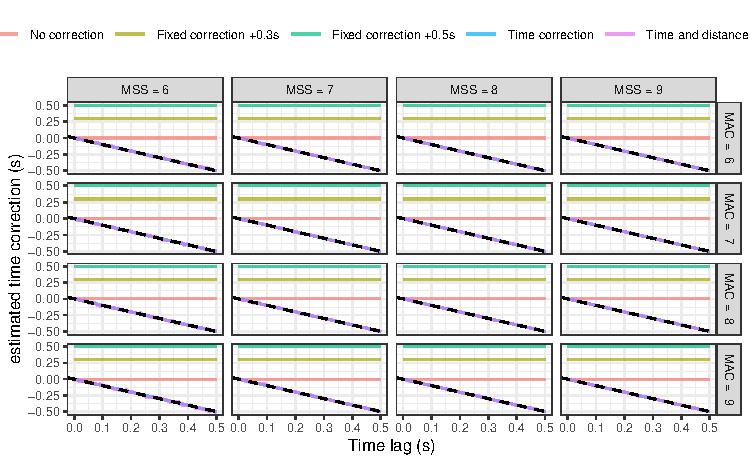
\includegraphics[width=1\linewidth]{paper_files/figure-latex/unnamed-chunk-46-1} \end{center}

\end{CodeChunk}

Here is the plot of the training and LOOCV residuals:

\begin{CodeChunk}
\begin{CodeInput}
R> df <- data.frame(
+   distance = jack_LOOCV$data$distance,
+   time = jack_LOOCV$data$time,
+   pred_time = jack_LOOCV$data$pred_time,
+   LOOCV_time = jack_LOOCV$LOOCV$data$pred_time
+ )
R> 
R> df <- df %>%
+   pivot_longer(cols = c("pred_time", "LOOCV_time"))
R> 
R> df$resid <- df$value - df$time
R> 
R> ggplot(df, aes(x = distance, y = resid, color = name)) +
+   theme_bw(8) +
+   geom_hline(yintercept = 0, linetype = "dashed") +
+   geom_point() +
+   theme(legend.title = element_blank()) +
+   xlab("Distance (m)") +
+   ylab("Predicted - observed time (s)") +
+   theme(
+     legend.title = element_blank(),
+     legend.position = "top")
\end{CodeInput}


\begin{center}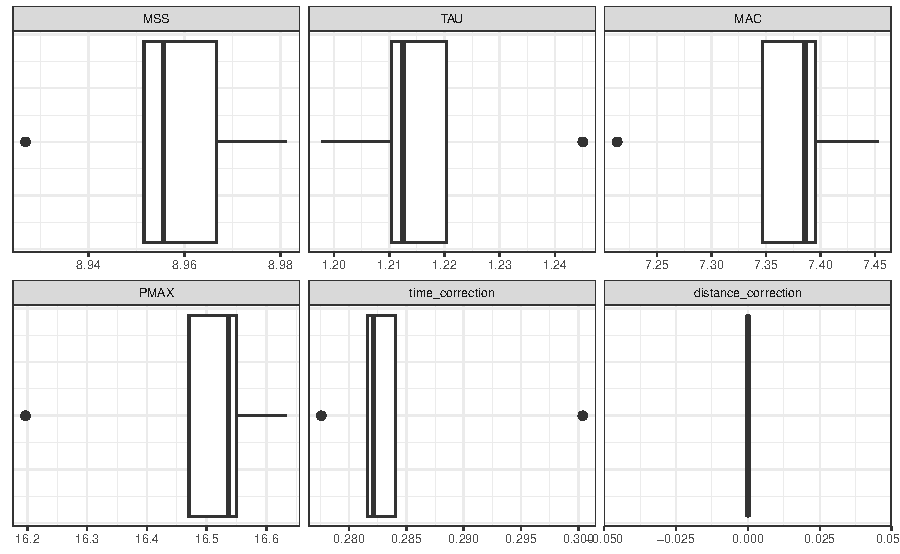
\includegraphics[width=1\linewidth]{paper_files/figure-latex/unnamed-chunk-47-1} \end{center}

\end{CodeChunk}

As expected, the model has more issues predicting unseen short or long sprints. Please note, that since LOOCV removes one observation, if the model estimates three parameters, then at least five observations are needed, since we need to make sure the model can be estimated once a single observation is removed. LOOCV can also be implemented with the mixed-effects models in the \pkg{shorts} package.

\hypertarget{example-analysis}{%
\section{Example analysis}\label{example-analysis}}

Let's utilize demonstrated functionalities of the \pkg{shorts} package using real-world data. The first dataset comes from Usain Bolt's performance from IAAF World Championship held in London, 2017, and the second dataset involve Jason Vescovi's sample data for 52 female soccer and field hockey athletes which comes with the \pkg{shorts} package (see \texttt{?vescovi}).

\hypertarget{usain-bolts-run-from-london-2017}{%
\subsection{Usain Bolt's run from London 2017}\label{usain-bolts-run-from-london-2017}}

The following dataset represents Usain Bolt's race in the finals at the IAAF World Championship held in London, 2017. Since reaction time enters the splits, we want to see how that will affect the model estimates, and particularly, if the estimated time correction model will pick-up reaction time.

For the sake of this analysis, only 10m splits over 60m are used.

\begin{CodeChunk}
\begin{CodeInput}
R> bolt_reaction_time <- 0.183
R> 
R> bolt_distance <- c(10, 20, 30, 40, 50, 60)
R> bolt_time <- c(1.963, 2.983, 3.883, 4.763, 5.643, 6.493)
R> 
R> # No corrections model
R> bolt_m1 <- model_using_splits(
+   distance = bolt_distance,
+   time = bolt_time
+ )
R> 
R> # Model with reaction time as fixed time correction
R> bolt_m2 <- model_using_splits(
+   distance = bolt_distance,
+   time = bolt_time,
+   time_correction = -bolt_reaction_time
+ )
R> 
R> # Model with estimated time correction
R> bolt_m3 <- model_using_splits_with_time_correction(
+   distance = bolt_distance,
+   time = bolt_time
+ )
R> 
R> # Model with estimated time correction, but deducted reaction time
R> bolt_m4 <- model_using_splits_with_time_correction(
+   distance = bolt_distance,
+   time = bolt_time - bolt_reaction_time
+ )
R> 
R> # Model with estimated time and distance corrections
R> bolt_m5 <- model_using_splits_with_corrections(
+   distance = bolt_distance,
+   time = bolt_time
+ )
R> 
R> # Model with estimated time and distance corrections and deducted reaction time
R> bolt_m6 <- model_using_splits_with_corrections(
+   distance = bolt_distance,
+   time = bolt_time - bolt_reaction_time
+ )
R> 
R> bolt_model <- rbind(
+   data.frame(
+     model = "No correction",
+     t(coef(bolt_m1))
+   ),
+   data.frame(
+     model = "No correction - RT",
+     t(coef(bolt_m2))
+   ),
+   data.frame(
+     model = "Time correction",
+     t(coef(bolt_m3))
+   ),
+   data.frame(
+     model = "Time correction - RT",
+     t(coef(bolt_m4))
+   ),
+   data.frame(
+     model = "Distance correction",
+     t(coef(bolt_m5))
+   ),
+   data.frame(
+     model = "Distance correction - RT",
+     t(coef(bolt_m6))
+   )
+ )
R> 
R> bolt_model
\end{CodeInput}
\begin{CodeOutput}
#>                      model  MSS   TAU   MAC PMAX time_correction
#> 1            No correction 12.1 1.564  7.77 23.6         0.00000
#> 2       No correction - RT 11.7 1.205  9.74 28.6        -0.18300
#> 3          Time correction 11.7 1.202  9.76 28.6        -0.18483
#> 4     Time correction - RT 11.7 1.202  9.76 28.6        -0.00183
#> 5      Distance correction 11.6 0.855 13.56 39.3        -0.81151
#> 6 Distance correction - RT 11.6 0.855 13.56 39.3        -0.62851
#>   distance_correction
#> 1                0.00
#> 2                0.00
#> 3                0.00
#> 4                0.00
#> 5               -3.98
#> 6               -3.98
\end{CodeOutput}
\end{CodeChunk}

\hypertarget{vescovi-data}{%
\subsection{Vescovi data}\label{vescovi-data}}

The data from Vescovi represents a sub-set of data from a total of 220 high-level female athletes (151 soccer players and 69 field hockey players). Using a random number generator, a total of 52 players (35 soccer and 17 field hockey) were selected for the sample dataset.

The protocol for assessing linear sprint speed has been described previously \citep{vescoviImpactMaximumSpeed2014, vescoviLocomotorHeartRateMetabolic2016, vescoviSprintSpeedCharacteristics2012} and was identical for each cohort. Briefly, all athletes performed a standardized warm-up that included general exercises such as jogging, shuffling, multi-directional movements, and dynamic stretching exercises. Infrared timing gates (Brower Timing, Utah) were positioned at the start line and at 5, 10, 20, 30, and 35 meters at a height of approximately 1.0 meter. Participants stood with their lead foot positioned approximately 5 cm behind the initial infrared beam (i.e., start line). Only forward movement was permitted (no leaning or rocking backwards) and timing started when the laser of the starting gate was triggered. The best 35 m time, and all associated split times were kept for analysis.

Below is the mixed-effects models analysis of the dataset.

\begin{CodeChunk}
\begin{CodeInput}
R> data("vescovi")
R> 
R> # Convert data to long
R> df <- vescovi %>%
+   select(1:13) %>%
+   # slice(1:10) %>%
+   pivot_longer(
+     cols = 9:13,
+     names_to = "distance",
+     values_to = "time"
+   ) %>%
+   mutate(
+     distance = as.numeric(str_extract(distance, "^[0-9]+"))
+   )
\end{CodeInput}
\end{CodeChunk}

The following models were used: (1) no corrections model, (2) fixed time correction model (using 0.3s heuristic rule of thumb), (3) estimated time correction as a fixed effect model, (4) estimated time correction as a random effect model, (5) estimated distance correction as fixed effect model (and time correction as random effect), and (6) estimated distance correction as random effect model.

\begin{CodeChunk}
\begin{CodeInput}
R> no_corrections <- mixed_model_using_splits(
+   df,
+   distance = "distance",
+   time = "time",
+   athlete = "Athlete"
+ )
R> 
R> fixed_correction <- mixed_model_using_splits(
+   df,
+   distance = "distance",
+   time = "time",
+   athlete = "Athlete",
+   time_correction = 0.3
+ )
R> 
R> time_correction_fixed <- mixed_model_using_splits_with_time_correction(
+   df,
+   distance = "distance",
+   time = "time",
+   athlete = "Athlete",
+   random = MSS + TAU ~ 1
+ )
R> 
R> time_correction_random <- mixed_model_using_splits_with_time_correction(
+   df,
+   distance = "distance",
+   time = "time",
+   athlete = "Athlete",
+   random = MSS + TAU + time_correction ~ 1
+ )
R> 
R> time_distance_correction_fixed <- mixed_model_using_splits_with_corrections(
+   df,
+   distance = "distance",
+   time = "time",
+   athlete = "Athlete",
+   random = MSS + TAU + time_correction ~ 1
+ )
R> 
R> time_distance_correction_random <- mixed_model_using_splits_with_corrections(
+   df,
+   distance = "distance",
+   time = "time",
+   athlete = "Athlete",
+   random = MSS + TAU + time_correction + distance_correction ~ 1
+ )
\end{CodeInput}
\end{CodeChunk}

The following image represents model fit estimator RSE for each model. As can be seen, RSE is reduced the more flexible the model.

\begin{CodeChunk}
\begin{CodeInput}
R> model_fit <- rbind(
+   data.frame(
+     model = "No corrections",
+     t(unlist(no_corrections$model_fit))
+   ),
+   data.frame(
+     model = "Fixed correction +0.3s",
+     t(unlist(fixed_correction$model_fit))
+   ),
+   data.frame(
+     model = "Time correction fixed",
+     t(unlist(time_correction_fixed$model_fit))
+   ),
+   data.frame(
+     model = "Time correction random",
+     t(unlist(time_correction_random$model_fit))
+   ),
+   data.frame(
+     model = "Time and distance correction fixed",
+     t(unlist(time_distance_correction_fixed$model_fit))
+   ),
+   data.frame(
+     model = "Time and distance correction random",
+     t(unlist(time_distance_correction_random$model_fit))
+   )
+ )
R> 
R> model_fit$model <- factor(
+   model_fit$model,
+   levels = rev(c(
+     "No corrections",
+     "Fixed correction +0.3s",
+     "Time correction fixed",
+     "Time correction random",
+     "Time and distance correction fixed",
+     "Time and distance correction random"
+   ))
+ )
R> 
R> ggplot(model_fit, aes(x = RSE, y = model)) +
+   theme_bw(8) +
+   geom_point() +
+   xlab("RSE (s)") +
+   ylab(NULL)
\end{CodeInput}


\begin{center}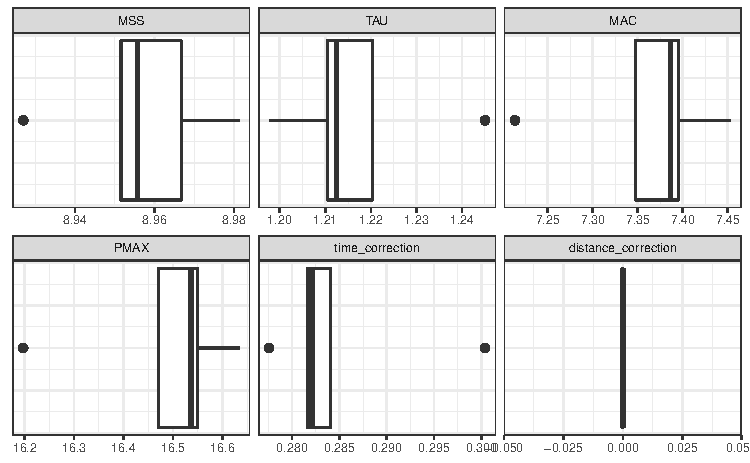
\includegraphics[width=1\linewidth]{paper_files/figure-latex/unnamed-chunk-51-1} \end{center}

\end{CodeChunk}

The following image depicts estimated parameters for each model:

\begin{CodeChunk}
\begin{CodeInput}
R> est_params <- rbind(
+   data.frame(
+     model = "No corrections",
+     no_corrections$parameters$random
+   ),
+   data.frame(
+     model = "Fixed correction +0.3s",
+     fixed_correction$parameters$random
+   ),
+   data.frame(
+     model = "Time correction fixed",
+     time_correction_fixed$parameters$random
+   ),
+   data.frame(
+     model = "Time correction random",
+     time_correction_random$parameters$random
+   ),
+   data.frame(
+     model = "Time and distance correction fixed",
+     time_distance_correction_fixed$parameters$random
+   ),
+   data.frame(
+     model = "Time and distance correction random",
+     time_distance_correction_random$parameters$random
+   )
+ )
R> 
R> est_params$model <- factor(
+   est_params$model,
+   levels = rev(c(
+     "No corrections",
+     "Fixed correction +0.3s",
+     "Time correction fixed",
+     "Time correction random",
+     "Time and distance correction fixed",
+     "Time and distance correction random"
+   ))
+ )
R> 
R> est_params <- est_params %>%
+   pivot_longer(cols = -(1:2), names_to = "parameter")
R> 
R> est_params$parameter <- factor(
+   est_params$parameter,
+   levels = c(
+     "MSS",
+     "TAU",
+     "MAC",
+     "PMAX",
+     "time_correction",
+     "distance_correction"
+   )
+ )
R> 
R> ggplot(est_params, aes(y = model, x = value)) +
+   theme_bw(8) +
+   geom_boxplot() +
+   facet_wrap(~parameter, scales = "free_x") +
+   xlab(NULL) +
+   ylab(NULL)
\end{CodeInput}


\begin{center}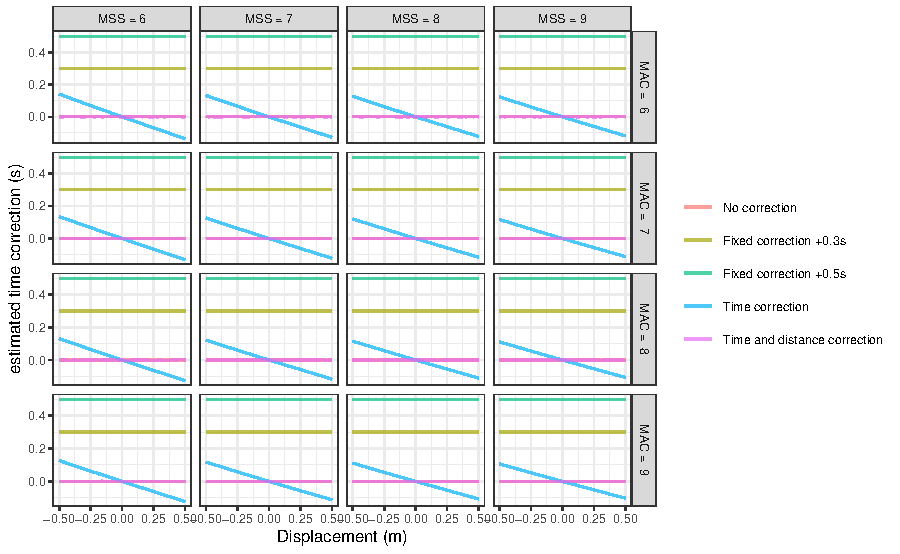
\includegraphics[width=1\linewidth]{paper_files/figure-latex/unnamed-chunk-52-1} \end{center}

\end{CodeChunk}

The following image depicts model residuals across distance splits. To provide practical magnitude of the residuals, we have used between subject observed time SD multiplied with 0.2 and -0.2. This provides practical anchor for the residual magnitude, often referred to as \emph{smallest worthwhile change} (SWC) or \emph{smallest effect size of interest} (SESOI) \citep{jovanovicBmbstatsBootstrapMagnitudebased2020}. If the residuals are within this magnitude band, then the model is good in making practically useful predictions.

Error bars represent residual bias \(\pm\) 1SD.

\begin{CodeChunk}
\begin{CodeInput}
R> model_resid <- rbind(
+   data.frame(
+     model = "No corrections",
+     no_corrections$data
+   ),
+   data.frame(
+     model = "Fixed correction +0.3s",
+     fixed_correction$data
+   ),
+   data.frame(
+     model = "Time correction fixed",
+     time_correction_fixed$data
+   ),
+   data.frame(
+     model = "Time correction random",
+     time_correction_random$data
+   ),
+   data.frame(
+     model = "Time and distance correction fixed",
+     time_distance_correction_fixed$data
+   ),
+   data.frame(
+     model = "Time and distance correction random",
+     time_distance_correction_random$data
+   )
+ )
R> 
R> 
R> model_resid$model <- factor(
+   model_resid$model,
+   levels = rev(c(
+     "No corrections",
+     "Fixed correction +0.3s",
+     "Time correction fixed",
+     "Time correction random",
+     "Time and distance correction fixed",
+     "Time and distance correction random"
+   ))
+ )
R> 
R> model_resid$resid <- model_resid$pred_time - model_resid$time
R> 
R> # Create SWC / SESOI band
R> model_SESOI <- model_resid %>%
+   group_by(model, distance) %>%
+   summarise(
+     bias = mean(resid),
+     variance = sd(resid),
+     upper = bias + variance,
+     lower = bias - variance,
+     MAD = mean(abs(resid)),
+     SESOI_upper = sd(time) * 0.2,
+     SESOI_lower = -sd(time) * 0.2
+   )
R> 
R> # Plot
R> ggplot(model_resid, aes(y = model)) +
+   theme_bw(8) +
+   geom_vline(
+     data = model_SESOI,
+     aes(xintercept = SESOI_lower),
+     color = "blue", alpha = 0.5, linetype = "dashed"
+   ) +
+   geom_vline(
+     data = model_SESOI,
+     aes(xintercept = SESOI_upper),
+     color = "blue", alpha = 0.5, linetype = "dashed"
+   ) +
+   geom_vline(xintercept = 0, color = "blue", alpha = 0.5) +
+   geom_jitter(aes(x = resid), alpha = 0.1, height = 0.25) +
+   geom_errorbarh(
+     data = model_SESOI,
+     aes(xmin = lower, xmax = upper),
+     height = 0.1, color = "black"
+   ) +
+   geom_point(data = model_SESOI, aes(x = bias), color = "black") +
+   facet_wrap(~distance, scales = "free_x") +
+   xlab("Predicted time - observed time (s)") +
+   ylab(NULL)
\end{CodeInput}


\begin{center}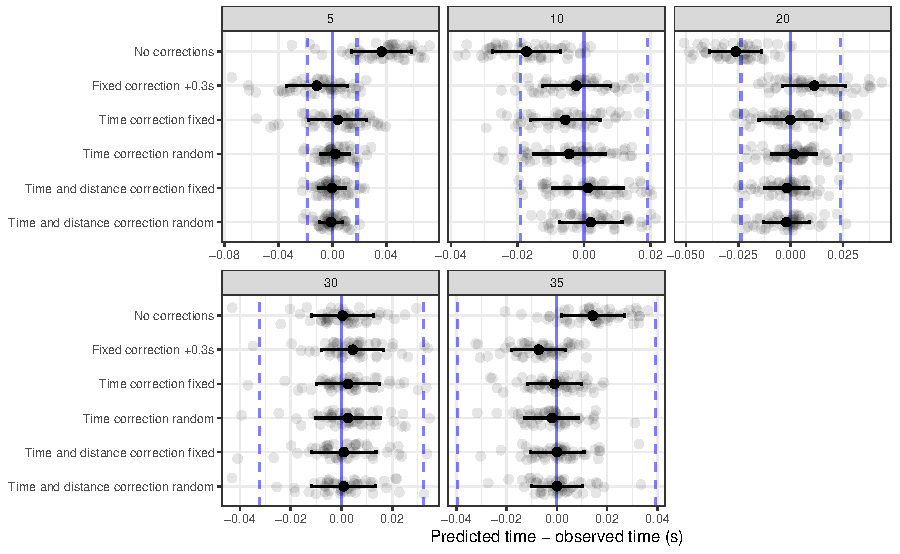
\includegraphics[width=1\linewidth]{paper_files/figure-latex/unnamed-chunk-53-1} \end{center}

\end{CodeChunk}

The following figure depicts model residuals estimators (bias, or mean residual; variance, or SD of the residuals, and MAD, or mean absolute difference).

\begin{CodeChunk}
\begin{CodeInput}
R> df <- model_SESOI %>%
+   pivot_longer(cols = -(1:2), names_to = "estimator") %>%
+   filter(estimator %in% c("bias", "variance", "MAD"))
R> 
R> df$model <- factor(
+   df$model,
+   levels = rev(c(
+     "No corrections",
+     "Fixed correction +0.3s",
+     "Time correction fixed",
+     "Time correction random",
+     "Time and distance correction fixed",
+     "Time and distance correction random"
+   ))
+ )
R> 
R> df$estimator <- factor(
+   df$estimator,
+   levels = c("bias", "variance", "MAD")
+ )
R> 
R> ggplot(df, aes(x = value, y = model)) +
+   theme_bw(8) +
+   geom_point() +
+   facet_grid(distance ~ estimator, scales = "free_x") +
+   xlab(NULL) +
+   ylab(NULL)
\end{CodeInput}


\begin{center}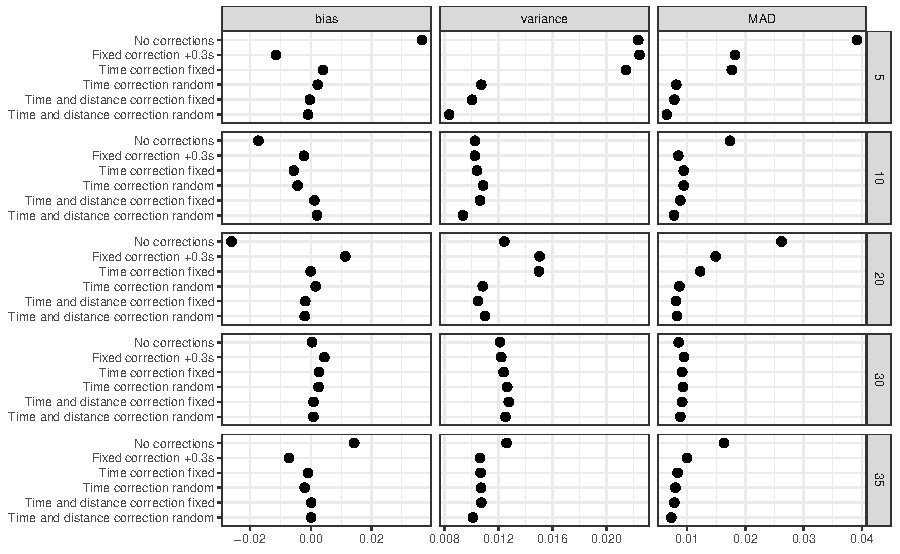
\includegraphics[width=1\linewidth]{paper_files/figure-latex/unnamed-chunk-54-1} \end{center}

\end{CodeChunk}

Which model should should be used? Although providing a better fit (using RSE as an estimator of model fit), the time and distance correction models often estimate these parameters that are harder to interpret (e.g., negative distance correction). Although providing novel theoretical models in this paper, we acknowledge the need for validating them in practice, against gold-standard methods, assessing their agreement, as well as their power in detecting and adjusting for timing inconsistencies.

We are hoping that the \pkg{shorts} package will help fellow sports scientists and coaches in exploring short sprint profiles and help in driving research, particularly in devising measuring protocols that are sensitive enough to capture training intervention changes, but also robust enough to take into account potential sprint initiation and timing inconsistencies.

\renewcommand\refname{References}
\bibliography{references.bib,packages.bib}


\end{document}
